%sección IV
\section{Método de revisión}\label{sec:metodo-revision}
Con el fin de alcanzar los objetivos propuestos para este articulo, se usó un acercamiento metodológico basado en que siguen Sepúlveda et al [Referencia del articulo de Sepúlveda] para construir un estudio de mapeo sistemático (SMS por sus siglas en inglés) basado en evidencia.

De acuerdo a los estudios [Sepulveda's article citations 16 and 17], es posible usar una combinación de estrategias de búsqueda para crear un SMS. Debido a esto, se ha decidido mezclar dos estrategias de búsqueda, una automática y la otra manual, para el mapeo sistemático propuesto en este articulo. También, se ha usado la metodología propuesta por Ali et al [Sepulveda's article citations 18] como un ejemplo.

Por ultimo, se ha soportado el proceso de construcción de este SMS con la ayuda del software SMS-Builder. Este software es una aplicación web que se creó para ayudar a los investigadores a seguir el proceso de construcción de una adaptación del SMS propuesto por [Sepulveda's article citations 14], que cubre seis fases del proceso de construcción del mapeo sistemático 1) Planeación, 2) Búsqueda de estudios, 3) Análisis de calidad, 4) Recolección de datos, 5) Clasificación y análisis de estudios, 6) Resultados. Ver Figura \ref{figure:Stages}. Para el estudio propuesto en este articulo, se usó SMS-Builder para guardar, procesar, analizar y evaluar los estudios a ser incluidos en el SMS [Sepulveda's article citations 19]. La herramienta puede ser encontrada en GitHub como software libre bajo la licencia GNU/GPL v3 en el siguiente link: https://github.com/grid-uq/sms-builder [Sepulveda's article citations 19].

\begin{figure}[htbp]
	\centering
	\includegraphics[width=0.6\linewidth]{resources/figures/sms-Etapas.drawio.png}
	\caption{Etapas del proceso de construcción de un SMS}
	\label{figure:Stages}
\end{figure}

% ETAPAS
%subsección 4.1 
\subsection{Planeación}
En esta etapa, se estableció el propósito general de la investigación y se definieron las metas, así como las preguntas de investigación, métricas, criterios de clasificación, criterios de inclusión/exclusión y criterios de calidad de los estudios. Ver Figura~\ref{fig:etapa1}. \\

\begin{figure*}[tbp]
    \centering
    \includegraphics[width=0.8\textwidth]{resources/images/planeacion/etapa1.png}
    \caption{Composición de la etapa de planeación}\label{fig:etapa1}
\end{figure*}

\subsubsection{Objetivos}
\mbox{}\\
Teniendo en cuenta los aspectos descritos en la sección de motivación, se definieron 2 metas generales para la revisión sistemática de la literatura que se presentan en el cuadro~\ref{tab:metas}.

\begin{table}[htbp]
    \centering
    \begin{tabular}{>{\centering\arraybackslash}m{1cm} >{\arraybackslash}m{7cm}}
        \hline
        \textbf{Goal} & \textbf{Description} \\
        \hline
        M1 & Identificar trabajos relacionados con VBC en proyectos de docencia, investigación y extensión. \\
        \\
        M2 & Clasificar trabajos relacionados con VBC en los dominios de desarrollo de software, pensamiento computacional, computación paralela, análisis de datos, inteligencia artificial, redes computacionales, infraestructura de TI, HPC, entre otros. \\
        
        \hline
    \end{tabular}
    \caption{Metas del estudio}\label{tab:metas}
\end{table}





\subsubsection{Pregunta de investigación}
\mbox{}

\begin{table}[tbp]
    \scriptsize % reduce tamaño del texto
    \centering
    \renewcommand{\arraystretch}{1.3}
    \begin{tabularx}{\columnwidth}{>{\centering\arraybackslash}m{0.18\columnwidth} >{\RaggedRight\arraybackslash}X}
        \hline
        \textbf{Aspecto} & \textbf{Descripción} \\
        \hline
        Población & Trabajos relacionados con la VBC aplicadas en diversos dominios de TI con un énfasis en la educación, investigación y extensión. \\
        Intervención & Identificación y clasificación de los trabajos en VBC en los dominios de TI establecidos. \\
        Comparación & 
        1. Se comparan los proyectos que han hecho uso de la VBC para determinar cuáles han tenido mayor tasa de éxito expresado por los autores en cada dominio de TI. \newline
        2. Se analiza el impacto de la VBC en proyectos de docencia, investigación y extensión en comparación con otras soluciones tecnológicas. \\
        Salida & Estructura de clasificación de los trabajos relacionados con las VBC en cada dominio de TI que han impactado en proyectos de docencia, investigación y extensión. \\
        Contexto & Docencia, investigación y extensión con apropiación de los dominios de TI en forma de VBC. \\
        \hline
    \end{tabularx}
    \caption{Aspectos del modelo PICOC}\label{tab:PICOC}
\end{table}

\begin{table*}[!t]
\centering

\renewcommand{\arraystretch}{1.4}
\begin{tabularx}{\textwidth}{>{\centering\arraybackslash}m{0.05\textwidth} >{\centering\arraybackslash}m{0.05\textwidth} >{\RaggedRight\arraybackslash}X >{\RaggedRight\arraybackslash}X}
\toprule
\textbf{Meta} & \textbf{Pregunta} & \textbf{Descripción} & \textbf{Motivación} \\
\midrule
G1 & Q1 & ¿Cuáles son los trabajos relacionados con tecnologías de virtualización basadas en contenedores (VBC) que podrían impactar positivamente proyectos de docencia, investigación y extensión? & La transversalidad que ofrece la VBC, gracias a su reproducibilidad de entornos, permite estimular diferentes aristas de la sociedad. Su naturaleza facilita el transporte de soluciones de TI entre diferentes entornos, generando que una innovación en cualquier dominio social impacte directamente en otro. \\
\midrule
G2 & Q2 & ¿Cuáles son los principales trabajos relacionados con las tecnologías de virtualización basadas en contenedores (VBC) que podrían contribuir en los diversos dominios de TI, entre los que pueden ser desarrollo de software, pensamiento computacional, computación paralela, análisis de datos, inteligencia artificial, redes computacionales, infraestructura de TI, HPC, entre otros? & Se busca proporcionar una base sólida para investigadores, docentes y profesionales interesados en comprender el estado del arte actual en relación con las VBC, además del alcance y las aplicaciones de estos trabajos sin necesidad de un análisis profundo. \\
\bottomrule
\end{tabularx}
\caption{Preguntas de investigación y su motivación}
\label{tab:preguntas}
\end{table*}

Este modelo permite establecer los aspectos de ``Población'', ``Intervención'', ``Comparación'', ``Salida'' y ``Contexto'' que sirven para situar el trabajo a realizar. Ver cuadro~\ref{tab:PICOC}. \\
\\
Teniendo en cuenta el modelo PICOC, se definieron las preguntas de investigación. Ver cuadro~\ref{tab:preguntas}.\\

\subsubsection{Métricas}
\mbox{}\\

\begin{table}[htbp]
\centering
\renewcommand{\arraystretch}{1.3}
\begin{tabularx}{\columnwidth}{>{\centering\arraybackslash}m{0.15\textwidth} >{\RaggedRight\arraybackslash}X}
\toprule
\textbf{Métrica} & \textbf{Descripción} \\
\midrule
M1 & Cantidad de trabajos identificados en cada dominio de TI. \\
M2 & Cantidad de trabajos que están incluidos en educación. \\
M3 & Cantidad de trabajos que están incluidos en investigación. \\
M4 & Cantidad de trabajos que están incluidos en extensión. \\
\bottomrule
\end{tabularx}
\caption{Métricas definidas para el análisis}
\label{tab:metricas}
\end{table}

Se definieron las métricas del estudio usando un enfoque cuantitativo de acuerdo con la estructura de clasificación. Los detalles de las métricas se presentan en el cuadro~\ref{tab:metricas}.
Los criterios determinados limitaron la validez de los documentos a tres años, buscando la actualidad en el estudio. Además, el tipo se limitó a estudios primarios, buscando un rigor mayor en la revisión por pares.\\

\subsubsection{Tópicos de investigación}
\mbox{}\\
Las preguntas de investigación y el modelo PICOC sirven como línea base para definir los tópicos de investigación que se consideran relevantes para el estudio. Estos tópicos son: \textit{Container-based virtualization}, \textit{Education}, \textit{Research}, \textit{Industry}. 
La definición de los tópicos de investigación se realizó teniendo en cuenta los dominios de TI que se consideraron relevantes para el estudio.\\

\subsubsection{Criterios de inclusión y exclusión}
\mbox{}\\
\begin{table*}[!t]
\centering
\renewcommand{\arraystretch}{1.4}
\begin{tabularx}{\textwidth}{>{\centering\arraybackslash}m{0.15\textwidth} >{\RaggedRight\arraybackslash}X >{\RaggedRight\arraybackslash}X}
\toprule
\textbf{Categoría} & \textbf{Inclusión} & \textbf{Exclusión} \\
\midrule
Campos & Abstract & -- \\
\midrule
Tipo de publicación & Journal articles and conference proceedings & Thesis and book chapters \\
\midrule
Área/Disciplina & Management, Computer Science, Information Technology and Management, Engineering & Areas not related to virtualization, Computer Science, and Information Technology and Management \\
\midrule
Período & Between 2022 to 2024 & Less than 2022 \\
\midrule
Idioma & English & -- \\
\bottomrule
\end{tabularx}
\caption{Criterios de inclusión y exclusión}\label{tab:criterios}
\end{table*}

Los criterios de inclusión y exclusión se definieron para garantizar que los estudios seleccionados sean relevantes para las preguntas de investigación y los objetivos del estudio. Los criterios se presentan en el cuadro~\ref{tab:criterios}.
Se definió un período de 3 años en busca de la actualidad de los estudios. Además, se limitó los estudios a artículos de revistas buscando un mayor rigor en la revisión por pares. Los estudios deben estar escritos en inglés y en las áreas de \textit{Computer Science} y \textit{Management}, \textit{Information Technology and Management}, \textit{Engineering} en busca de la calidad de los estudios. Finalmente, se excluyeron los estudios que no están relacionados con la VBC, que no son revisados por pares o que no están disponibles en línea.\\

\subsubsection{Criterios de calidad}
\mbox{}\\
Para finalizar la etapa de planeación, se definieron tres criterios de calidad. \\

El primer criterio de calidad es una adaptación del CVI (Content Value Index)~\cite{almanasreh2019evaluation} y~\cite{yaghmaei2003content}.
En este caso, los artículos se evaluaron para determinar si cumplen con los criterios de inclusión y exclusión definidos y si son relevantes para las preguntas de investigación. Se usó una escala cuantitativa de 0 a 5, donde 0 indica una baja relación con las metas del SMS y 5 indica una alta relación.
Ver formula~\ref{eq:cvi}. En esta formula, K es el número impar de evaluadores y f(n) es la frecuencia de respuestas para cada valor de la escala.\\

\begin{equation}
\label{eq:cvi}
CVI = \frac{\sum_{n=1}^{k} f(n)}{k}
\end{equation}

El segundo criterio de calidad es el número de citas de cada estudio de acuerdo con la fecha de publicación (A), el cual se denomina SCI (Scientific Citation Index). Ver formula~\ref{eq:sci}. En esta formula, C es el número de citas entre 2022 y 2024 y A es el tiempo de publicación del estudio. Así, un artículo publicado en 2024 con las misma cantidad de citas que un artículo publicado en 2022 tendrá un SCI más alto.\\

\begin{equation}
\label{eq:sci}
SCI = \frac{C}{A}
\end{equation}

El tercer criterio de calidad corresponde a la relación de los estudios con las preguntas de investigación. Este criterio se denomina IRRQ (Indice de relación con las preguntas de investigación). Ver formula~\ref{eq:irrq}. 

\begin{equation}
\label{eq:irrq}
IRRQ = \frac{N}{2}
\end{equation}

N corresponde al número de preguntas de investigación que el estudio responde. Este valor se divide en 2 porque es el número de preguntas de investigación definidas en la etapa de planeación. \\

%subsección 4.2
% subseccion 4.2
\subsection{Etapa 2: Búsqueda de Estudios}
Esta etapa presenta la estrategia de búsqueda usada en la revisión sistemática de la literatura. Esta estrategia se describe en detalle en las subsecciones~\ref{subsubsec:Definiendo la Estrategia de Busqueda} -- \ref{subsubsec:resultados-busqueda}. Ver figura~\ref{fig:etapa2}.

\begin{figure*}[tbp]
    \centering
    \includegraphics[width=0.8\textwidth]{resources/images/planeacion/estrategias-busqueda.png}
    \caption{Composición de la etapa de búsqueda de estudios}\label{fig:etapa2}
\end{figure*}
\mbox{}\\

%sub-subseccion 4.2.1 
\subsubsection{Definiendo la Estrategia de Búsqueda}\label{subsubsec:Definiendo la Estrategia de Busqueda}
\mbox{}\\
% Content for 4.2.1
Para la construcción de esta revisión de la literatura, se usó un enfoque híbrido. Con este enfoque se busca obtener mayor volumen de artículos indexados y con diferentes origenes. más allá de los proporcionados por las bases de datos.
En este sentido, se combinaron dos estrategias de búsqueda. La primer estrategia es la búsqueda en bases de datos y consiste en realizar una cadena de búsqueda automatizada en bases de datos académicas.~\cite{jalali2012systematic}.
La segunda estrategia es la denominada ``Bola de Nieve'' (Snowballing) y consiste en la búsqueda manual de artículos a partir de un conjunto base de artículos usando las referencias y las citas de los mismos. Esta estrategia se basa en la premisa de que los artículos relevantes citan otros artículos relevantes y, por lo tanto, permite encontrar artículos que no están indexados en las bases de datos académicas.~\cite{jalali2012systematic} y \cite{goodman1961snowball}.
\mbox{}\\
%sub-subseccion 4.2.2

\subsubsection{Estrategia de Búsqueda 1: Bases de Datos}
\mbox{}\\
Esta estrategia consta de 2 componentes. El primer componente es denominado ``Identificación de estudios''. Esto se enfoca en definir las palabras clave para construir las cadenas de búsqueda que conducen a completar las búsquedas en las bases de datos académicas.
El segundo componente es llamado ``Selección de estudios''. Se enfoca en aplicar varios criterios para refinar la búsqueda de resultados de estudios y así obtener el mayor valor del proceso de búsqueda. \\ \\

\begin{itemize}
    \item \textbf{Identificación de estudios:} En búsqueda de la viabilidad del estudio y por acuerdo de los autores, se limitó la búsqueda a cinco bases de datos académicas: \textit{ACM}, \textit{IEEE Xplore}, \textit{Springer}, \textit{Science Direct} y \textit{Taylor and Francis}. En esta parte del proceso es necesario establecer las palabras claves definidas antes y construir las cadenas de búsqueda específica para cada base de datos. Nuevamente se usó el modelo PICOC como guía metodológica para identificar términos claves o frases completas que se relacionan con las tecnologías de virtualización basadas en contenedores. En la construcción de estas cadenas de búsqueda se usaron sinónimos para ampliar el espectro de resultados. (Ver cuadro~\ref{tab:palabras-clave}).\\ 
    Las principales palabras clave identificadas fueron: \textit{Container-based virtualization}, \textit{Education}, \textit{Research}, \textit{Industry}. Para ampliar y refinar los resultados se usaron operadores booleanos como \textit{AND} y \textit{OR}. Además, se usaron comillas para buscar frases completas y paréntesis para agrupar términos relacionados. Finalmente, el conjunto de palabras clave seleccionadas para construir las cadenas de búsqueda se presenta en el cuadro~\ref{tab:keywords}.\\
    Para dirigir la búsqueda hacia la intercepción de los dominios de TI y la VBC se usó el operador booleano \textit{AND}. Una vez identificadas las palabras clave, se procedió con la construcción de las cadenas de búsqueda para cada base de datos, usando un proceso iterativo. El proceso de construcción de las cadenas de búsqueda consitió en realizar un proceso heúristico con las palabras clave, sinónimos y conceptos relacionados, haciendo uso de conjunciones y disyunciones conforme a las reglas de cada base de datos.\\ 
    Así, estas cadenas de búsqueda varían de acuerdo con las reglas de cada base de datos. Ver cuadro~\ref{tab:cadenas-busqueda}.\\

\end{itemize}

\begin{table}[tbp]
    \scriptsize % reduce tamaño del texto
    \centering
    \renewcommand{\arraystretch}{1.3}
    \begin{tabularx}{\columnwidth}{>{\centering\arraybackslash}m{0.18\columnwidth} >{\RaggedRight\arraybackslash}X}
        \hline
        \textbf{Aspecto} & \textbf{Descripción} \\
        \hline
        Población & VBC, Dominios de TI, Educación, Investigación, Extensión \\
        Intervención & Identificación, Clasificación \\
        Comparación & Tasa de éxito, Evidencia de uso \\
        Salida & Clasificación de trabajos relacionados con VBC en cada dominio de TI \\
        Contexto & Docencia, Investigación, Extensión \\
        \hline
    \end{tabularx}
    \caption{Palabras clave identificadas usando el modelo PICOC}\label{tab:palabras-clave}
\end{table}

\begin{table}[tbp]
    \scriptsize % reduce tamaño del texto
    \centering
    \renewcommand{\arraystretch}{1.3}
    \begin{tabularx}{\columnwidth}{>{\centering\arraybackslash}m{0.18\columnwidth} >{\RaggedRight\arraybackslash}X}
        \hline
        \textbf{Palabras clave} & \textbf{Sinónimos} \\
        \hline
        Container-based virtualization & Application virtualization, Docker, Lightweight Virtualization \\
        Education & Education System, Education Development, Higher Education \\
        Research & Research Group, Research Proposal \\
        Industry & IT Services, Technology Infrastructure, Cloud Computing \\
        \hline
    \end{tabularx}
    \caption{Palabras clave para la búsqueda en base de datos}\label{tab:keywords}
\end{table}




\newcolumntype{P}[1]{>{\raggedright\arraybackslash}p{#1}}

\begin{sidewaystable*}[htbp]
\centering
\scriptsize
\renewcommand{\arraystretch}{1.5}
\begin{adjustbox}{max width=\textwidth}
\begin{tabular}{|P{0.18\linewidth}|P{0.20\linewidth}|P{0.20\linewidth}|P{0.20\linewidth}|P{0.20\linewidth}|P{0.20\linewidth}|}
\hline
\textbf{Dominio / Base de Datos} & \textbf{ACM Digital Library} & \textbf{IEEE Xplore} & \textbf{ScienceDirect} & \textbf{SpringerLink}  & \textbf{Taylor \& Francis} \\
\hline
\textbf{Educación AND VBC} 
& \tiny \texttt{(Title:(``Container-based virtualization'' OR ``Application virtualization'' OR ``Docker'' OR ``Lightweight Virtualization'') AND Title:(``Education'' OR ``Education System'' OR ``Education Development'' OR ``Higher Education'')) OR (Abstract:(``Container-based virtualization'' OR ``Application virtualization'' OR ``Docker'' OR ``Lightweight Virtualization'') AND Abstract:(``Education'' OR ``Education System'' OR ``Education Development'' OR ``Higher Education'')) OR (Keyword:(``Container-based virtualization'' OR ``Application virtualization'' OR ``Docker'' OR ``Lightweight Virtualization'') AND Keyword:(``Education'' OR ``Education System'' OR ``Education Development'' OR ``Higher Education''))} 
& \tiny \texttt{((``Abstract'': ``Container-based virtualization'' OR ``Abstract'': ``Application virtualization'' OR ``Abstract'': ``Docker'' OR ``Abstract'': ``Lightweight Virtualization'') AND (``Abstract'': ``Education'' OR ``Abstract'': ``Education System'' OR ``Abstract'': ``Education Development''  OR ``Abstract'': ``Higher Education'')) OR ((``Publication Title'': ``Container-based virtualization'' OR ``Publication Title'': ``Application virtualization'' OR ``Publication Title'': ``Docker'' OR ``Publication Title'': ``Lightweight Virtualization'') AND (``Publication Title'': ``Education'' OR ``Publication Title'': ``Education System'' OR ``Publication Title'': ``Education Development''  OR ``Publication Title'': ``Higher Education'')) OR ((``Author Keywords'': ``Container-based virtualization'' OR ``Author Keywords'': ``Application virtualization'' OR ``Author Keywords'': ``Docker'' OR ``Author Keywords'': ``Lightweight Virtualization'') AND (``Author Keywords'': ``Education'' OR ``Author Keywords'': ``Education System'' OR ``Author Keywords'': ``Education Development''  OR ``Author Keywords'': ``Higher Education''))} 
& \tiny \texttt{(``Container-based virtualization'' OR ``Application virtualization'' OR ``Docker'' OR ``Lightweight Virtualization'') AND (``Education'' OR ``Education System'' OR ``Education Development'' OR ``Higher Education'')} 
& \tiny \texttt{(title:(``Container-based virtualization'' OR ``Application virtualization'' OR ``Docker'' OR ``Lightweight Virtualization'') AND title:(``Education'' OR ``Education System'' OR ``Education Development'' OR ``Higher Education'')) OR (abstract:(``Container-based virtualization'' OR ``Application virtualization'' OR ``Docker'' OR ``Lightweight Virtualization'') AND abstract:(``Education'' OR ``Education System'' OR ``Education Development'' OR ``Higher Education'')) OR (keyword:(``Container-based virtualization'' OR ``Application virtualization'' OR ``Docker'' OR ``Lightweight Virtualization'') AND keyword:(``Education'' OR ``Education System'' OR ``Education Development'' OR ``Higher Education''))} 
& \tiny \texttt{(``Application virtualization'' OR ``Docker'' OR ``Lightweight Virtualization'' OR ``Docker Container'') AND (``Education System'' OR ``Education Sector'' OR ``Education Development'' OR ``Higher Education'')} \\
\hline

\hline
\textbf{Investigación AND VBC}
& \tiny \texttt{(Title:(``Container-based virtualization'' OR ``Application virtualization'' OR ``Docker'' OR ``Lightweight Virtualization'') AND Title:(``Research'' OR ``Research Group'' OR ``Research Proposal'')) OR (Abstract:(``Container-based virtualization'' OR ``Application virtualization'' OR ``Docker'' OR ``Lightweight Virtualization'') AND Abstract:(``Research'' OR ``Research Group'' OR ``Research Proposal'')) OR (Keyword:(``Container-based virtualization'' OR ``Application virtualization'' OR ``Docker'' OR ``Lightweight Virtualization'') AND Keyword:(``Research'' OR ``Research Group'' OR ``Research Proposal''))} 
& \tiny \texttt{((``Abstract'': ``Container-based virtualization'' OR ``Abstract'': ``Application virtualization'' OR ``Abstract'': ``Docker'' OR ``Abstract'': ``Lightweight Virtualization'') AND (``Abstract'': ``Research Group'' OR ``Abstract'': ``Research Proposal'')) OR ((``Publication Title'': ``Container-based virtualization'' OR ``Publication Title'': ``Application virtualization'' OR ``Publication Title'': ``Docker'' OR ``Publication Title'': ``Lightweight Virtualization'') AND (``Publication Title'': ``Research Group'' OR ``Publication Title'': ``Research Proposal'')) OR ((``Author Keywords'': ``Container-based virtualization'' OR ``Author Keywords'': ``Application virtualization'' OR ``Author Keywords'': ``Docker'' OR ``Author Keywords'': ``Lightweight Virtualization'') AND (``Author Keywords'': ``Research Group'' OR ``Author Keywords'': ``Research Proposal''))} 
& \tiny \texttt{(``Container-based virtualization'' OR ``Application virtualization'' OR ``Docker'' OR ``Lightweight Virtualization'') AND (``Research'' OR ``Research Group'' OR ``Research Proposal'')} 
& \tiny \texttt{(title:(``Container-based virtualization'' OR ``Application virtualization'' OR ``Docker'' OR ``Lightweight Virtualization'') AND title:(``Research'' OR ``Research Group'' OR ``Research Proposal'')) OR (abstract:(``Container-based virtualization'' OR ``Application virtualization'' OR ``Docker'' OR ``Lightweight Virtualization'') AND abstract:(``Research'' OR ``Research Group'' OR ``Research Proposal'')) OR (keyword:(``Container-based virtualization'' OR ``Application virtualization'' OR ``Docker'' OR ``Lightweight Virtualization'') AND keyword:(``Research'' OR ``Research Group'' OR ``Research Proposal''))} 
& \tiny \texttt{(``Application virtualization'' OR ``Docker'' OR ``Lightweight Virtualization'' OR ``Docker Container'') AND (``Specific Research Areas'' OR ``Research Group'' OR ``Research Proposal'' OR ``Research and Development'')} \\
\hline

\hline
\textbf{Industria AND VBC}
& \tiny \texttt{(Title:(``Container-based virtualization'' OR ``Application virtualization'' OR ``Docker'' OR ``Lightweight Virtualization'') AND Title:(``Industry'' OR ``IT Services'' OR ``Technology Infrastructure'' OR ``Cloud Computing'')) OR (Abstract:(``Container-based virtualization'' OR ``Application virtualization'' OR ``Docker'' OR ``Lightweight Virtualization'') AND Abstract:(``Industry'' OR ``IT Services'' OR ``Technology Infrastructure'' OR ``Cloud Computing'')) OR (Keyword:(``Container-based virtualization'' OR ``Application virtualization'' OR ``Docker'' OR ``Lightweight Virtualization'') AND Keyword:(``Industry'' OR ``IT Services'' OR ``Technology Infrastructure'' OR ``Cloud Computing''))} 
& \tiny \texttt{((``Abstract'': ``Container-based virtualization'' OR ``Abstract'': ``Application virtualization'' OR ``Abstract'': ``Docker'' OR ``Abstract'': ``Lightweight Virtualization'') AND (``Abstract'': ``Industry'' OR ``Abstract'': ``IT Services'' OR ``Abstract'': ``Technology Infrastructure'' OR ``Abstract'': ``Cloud Computing'')) OR ((``Publication Title'': ``Container-based virtualization'' OR ``Publication Title'': ``Application virtualization'' OR ``Publication Title'': ``Docker'' OR ``Publication Title'': ``Lightweight Virtualization'') AND (``Publication Title'': ``Industry'' OR ``Publication Title'': ``IT Services'' OR ``Publication Title'': ``Technology Infrastructure'' OR ``Publication Title'': ``Cloud Computing'')) OR ((``Author Keywords'': ``Container-based virtualization'' OR ``Author Keywords'': ``Application virtualization'' OR ``Author Keywords'': ``Docker'' OR ``Author Keywords'': ``Lightweight Virtualization'') AND (``Author Keywords'': ``Industry'' OR ``Author Keywords'': ``IT Services'' OR ``Author Keywords'': ``Technology Infrastructure'' OR ``Author Keywords'': ``Cloud Computing''))} 
& \tiny \texttt{(``Container-based virtualization'' OR ``Application virtualization'' OR ``Docker'' OR ``Lightweight Virtualization'') AND (``Industry'' OR ``IT Services'' OR ``Technology Infrastructure'' OR ``Cloud Computing'')} 
& \tiny \texttt{(title:(``Container-based virtualization'' OR ``Application virtualization'' OR ``Docker'' OR ``Lightweight Virtualization'') AND title:(``Industry'' OR ``IT Services'' OR ``Technology Infrastructure'' OR ``Cloud Computing'')) OR (abstract:(``Container-based virtualization'' OR ``Application virtualization'' OR ``Docker'' OR ``Lightweight Virtualization'') AND abstract:(``Industry'' OR ``IT Services'' OR ``Technology Infrastructure'' OR ``Cloud Computing'')) OR (keyword:(``Container-based virtualization'' OR ``Application virtualization'' OR ``Docker'' OR ``Lightweight Virtualization'') AND keyword:(``Industry'' OR ``IT Services'' OR ``Technology Infrastructure'' OR ``Cloud Computing''))} 
& \tiny \texttt{(``Application virtualization'' OR ``Docker'' OR ``Lightweight Virtualization'' OR ``Docker Container'') AND (``Industry'' OR ``IT Services'' OR ``Technology Infrastructure'' OR ``Cloud Computing'')} \\
\hline
\end{tabular}
\end{adjustbox}
\caption{Cadenas de búsqueda por dominio y base de datos}\label{tab:cadenas-busqueda}
\end{sidewaystable*}










% sub-subsetion for 4.2.3
\subsubsection{Estrategia de Búsqueda 2: Bola de Nieve (Snowballing)}
Quis ut deserunt in nulla aliquip exercitation. Voluptate non laborum do eu dolor mollit officia cupidatat do ea id id ullamco. Dolore velit anim est pariatur eiusmod occaecat duis labore reprehenderit nisi esse. Eu laboris cillum ullamco non velit veniam labore eiusmod laboris sint. Consequat officia aliquip velit officia do ex nulla cupidatat elit dolore deserunt sint.
\mbox{}\\

% sub=-subsection 4.2.4
\subsubsection{Resultados de la Búsqueda de Estudios}
\label{subsubsec:resultados-busqueda}
Nostrud enim magna culpa labore in culpa aliqua dolore ea amet sit magna exercitation sunt. Voluptate qui aliqua velit ipsum ullamco dolor ad velit cupidatat dolore sint. Nisi cillum dolore magna tempor minim ullamco anim quis ipsum consequat officia.
\mbox{}\\

%subsección 4.3
% subsection 4.3
\subsection{Stage 3: Quality Assessment}
According to~\cite{Ali-01}, the incorporation of a quality assessment is not mandatory in an SMS. However, such assessment could bring an SMS closer to a systematic review~\cite{Petersen-01}. Consequently, we sought to verify the relevance of the studies identified by the SMS objectives through this process. To carry out such assessment, the CVI (\textit{Content Value Index}), SCI (\textit{Study Citation Index}), and IRRQ (\textit{Index of Relationship to Research Questions}) indices defined during the planning stage were employed.

%sub-subsection 4.3.1
\subsubsection{Content Validity Assessment}
In this assessment, the content of the studies was analyzed to determine their value in the research context. For this purpose, the CVI index described in the planning stage was applied.

The rating of studies according to the CVI index was performed with the assistance of the SMS-Builder software. Subsequently, a frequency analysis was conducted to select the studies from the most significant quartile, that is, those with the highest CVI. This type of assessment is performed when identifying the \totalEtapaDos{} studies included in the SMS, whose results are presented in \hbox{Step 5: Study classification.}

%sub-subsection 4.3.2
\subsubsection{Index for Quality Assessment by Number of Citations}
The assessment of studies was performed by the team, taking into account the SCI index. We calculated this index with the support of the SMS-Builder software~\cite{sms-builder-repo} and citation data from Google Scholar. Subsequently, a frequency analysis was also conducted to select the studies from the most significant quartile, that is, those with the highest SCI.

%sub-subsection 4.3.3
\subsubsection{Index for the Evaluation of the Relationship of Studies to Research Questions}
This quality assessment uses the IRRQ index, described in the planning stage (Section~\ref{sec:planeacion}). In this regard, the selected studies were analyzed to establish their relationship with the classification topics.

Through this process, the SMS-Builder software~\cite{sms-builder-repo} was configured to establish the direct relationship of the studies with the research questions proposed in this SMS. As in the previous cases, a frequency analysis was also performed, where the quartile of most significant studies was selected, that is, those with the highest IRRQ.


%subsección 4.4
% subseccion 4.4
\subsection{Etapa 4: Extracción de Datos}\label{sec:extraccion-de-datos}

Una vez aplicados los procedimientos de búsqueda y selección de estudios, así como la evaluación de su calidad, se seleccionaron \totalEtapaDos{} estudios primarios. Estos estudios se etiquetaron con el prefijo SPS (Selected Primary Study) seguido de un número. La lista completa de estos estudios se encuentra en la Tabla \ref{table:selected_primary_studies}.

A partir de los \totalEtapaDos{} estudios primarios seleccionados (SPS), se diseñaron y completaron los formularios para obtener datos relevantes para la SMS. La información contenida en los SPSs se relacionó con las preguntas de investigación a través de los temas definidos en la fase de planificación y consignados mediante los modelos GQM y PICOC. Además, se extrajeron metadatos como palabras clave para identificar aspectos subyacentes de los SPSs.


% -------- Tabla : Estudios Primarios Seleccionados (SPSs) ------------
\begin{table*}[htbp]
	\centering
	\caption{Los \totalStudies{} estudios primarios seleccionados (SPSs)}
	\label{table:selected_primary_studies}
	\renewcommand{\arraystretch}{1.2}
	\setlength{\tabcolsep}{4pt} % Reduce space between columns
	\begin{tabular*}{\textwidth}{l @{\extracolsep{\fill}} r l @{\extracolsep{\fill}} r l @{\extracolsep{\fill}} r l @{\extracolsep{\fill}} r l @{\extracolsep{\fill}} r}
		\toprule
		\textbf{ID} & \textbf{Ref} & \textbf{ID} & \textbf{Ref} & \textbf{ID} & \textbf{Ref} & \textbf{ID} & \textbf{Ref} & \textbf{ID} & \textbf{Ref} \\
		\midrule
		SPS001      & [1]          & SPS002      & [2]          & SPS003      & [3]          & SPS004      & [4]          & SPS005      & [5]          \\
		SPS006      & [6]          & SPS007      & [7]          & SPS008      & [8]          & SPS009      & [9]          & SPS010      & [10]         \\
		SPS011      & [11]         & SPS012      & [12]         & SPS013      & [13]         & SPS014      & [14]         & SPS015      & [15]         \\
		SPS016      & [16]         & SPS017      & [17]         & SPS018      & [18]         & SPS019      & [19]         & SPS020      & [20]         \\
		SPS021      & [21]         & SPS022      & [22]         & SPS023      & [23]         & SPS024      & [24]         & SPS025      & [25]         \\
		SPS026      & [26]         & SPS027      & [27]         & SPS028      & [28]         & SPS029      & [29]         & SPS030      & [30]         \\
		SPS031      & [31]         & SPS032      & [32]         & SPS033      & [33]         & SPS034      & [34]         & SPS035      & [35]         \\
		SPS036      & [36]         & SPS037      & [37]         & SPS038      & [38]         & SPS039      & [39]         & SPS040      & [40]         \\
		SPS041      & [41]         & SPS042      & [42]         & SPS043      & [43]         & SPS044      & [44]         & SPS045      & [45]         \\
		SPS046      & [46]         & SPS047      & [47]         & SPS048      & [48]         & SPS049      & [49]         & SPS050      & [50]         \\
		SPS051      & [51]         & SPS052      & [52]         & SPS053      & [53]         & SPS054      & [54]         & SPS055      & [55]         \\
		SPS056      & [56]         & SPS057      & [57]         & SPS058      & [58]         & SPS059      & [59]         & SPS060      & [60]         \\
		SPS061      & [61]         & SPS062      & [62]         & SPS063      & [63]         & SPS064      & [64]         & SPS065      & [65]         \\
		SPS066      & [66]         & SPS067      & [67]         & SPS068      & [68]         & SPS069      & [69]         & SPS070      & [70]         \\
		SPS071      & [71]         & SPS072      & [72]         & SPS073      & [73]         & SPS074      & [74]         & SPS075      & [75]         \\
		SPS076      & [76]         & SPS077      & [77]         & SPS078      & [78]         & SPS079      & [79]         & SPS080      & [80]         \\
		SPS081      & [81]         & SPS082      & [82]         & SPS083      & [83]         & SPS084      & [84]         & SPS085      & [85]         \\
		SPS086      & [86]         & SPS087      & [87]         & SPS088      & [88]         & SPS089      & [89]         & SPS090      & [90]         \\
		SPS091      & [91]         & SPS092      & [92]         & SPS093      & [93]         & SPS094      & [94]         & SPS095      & [95]         \\
		SPS096      & [96]         & SPS097      & [97]         & SPS098      & [98]         & SPS099      & [99]         & SPS100      & [100]        \\
		SPS101      & [101]        & SPS102      & [102]        & SPS103      & [103]        & SPS104      & [104]        & SPS105      & [105]        \\
		SPS106      & [106]        & SPS107      & [107]        & SPS108      & [108]        & SPS109      & [109]        & SPS110      & [110]        \\
		SPS111      & [111]        & SPS112      & [112]        & SPS113      & [113]        & SPS114      & [114]        &             &              \\
		\bottomrule
	\end{tabular*}
\end{table*}
% --------------------------------------------------------------


El proceso fue respaldado por diversas herramientas informáticas, como hojas de cálculo, software especializado en la gestión de referencias bibliográficas (por ejemplo, EndNote y Mendeley), y SMS-Builder \cite{sms-builder-repo} para la construcción del análisis de datos. Toda la información de este SMS ha sido publicada en el sitio \cite{sms-builder-own-container}.

Los interesados pueden obtener un contenedor Docker \textcolor{red}{(!TODO Colocar el link del Dockerhub donde se encuentra alojado el contenedor con todo el SMS)} que incluye una versión funcional de SMS-Builder con todos los datos utilizados en este estudio. Se invita a los lectores a interactuar con esta herramienta tecnológica para obtener información complementaria a la que se presenta en este artículo.


%subsección 4.5
% subseccion 4.5
\subsection{Etapa 5: Clasificación de Estudios}\label{sec:clasificacion-estudios}
La clasificación de los SPS se realizó haciendo uso de tópicos de agrupamiento, como se observa en la tabla~\ref{}

%subsección 4.6
% subsection 4.6
\subsection{Stage 6: Results}
This section presents the results obtained through the execution of the SMS search protocol. Initially, a general description of the data corresponding to the Selected Primary Studies (SPSs) is provided.

This description covers aspects such as the origin of the studies, year of publication, search strategy, quality indices, their relationship with the research questions (RQs) and respective topics, and the keywords. Finally, a word cloud generated from the keywords of the SPSs is presented.

It is important to recall that the association between the SPSs and the topics was established through the detailed classification described in Section \ref{subsec:clasificacion-de-estudios}. Consequently, the RQs were also associated, since the topics follow a specific structure within them.

Furthermore, the association between the main SMS keywords and the section titles, abstracts, and keywords of all SPSs was identified.

% sub-subsection 4.6.1
\subsubsection{General Description of the SPSs (Selected Primary Studies)}
The process of searching and filtering studies resulted in the identification of 114 SPSs, as shown in Table \ref{table:selected_primary_studies}.

\begin{figure}[ht]
	\centering
	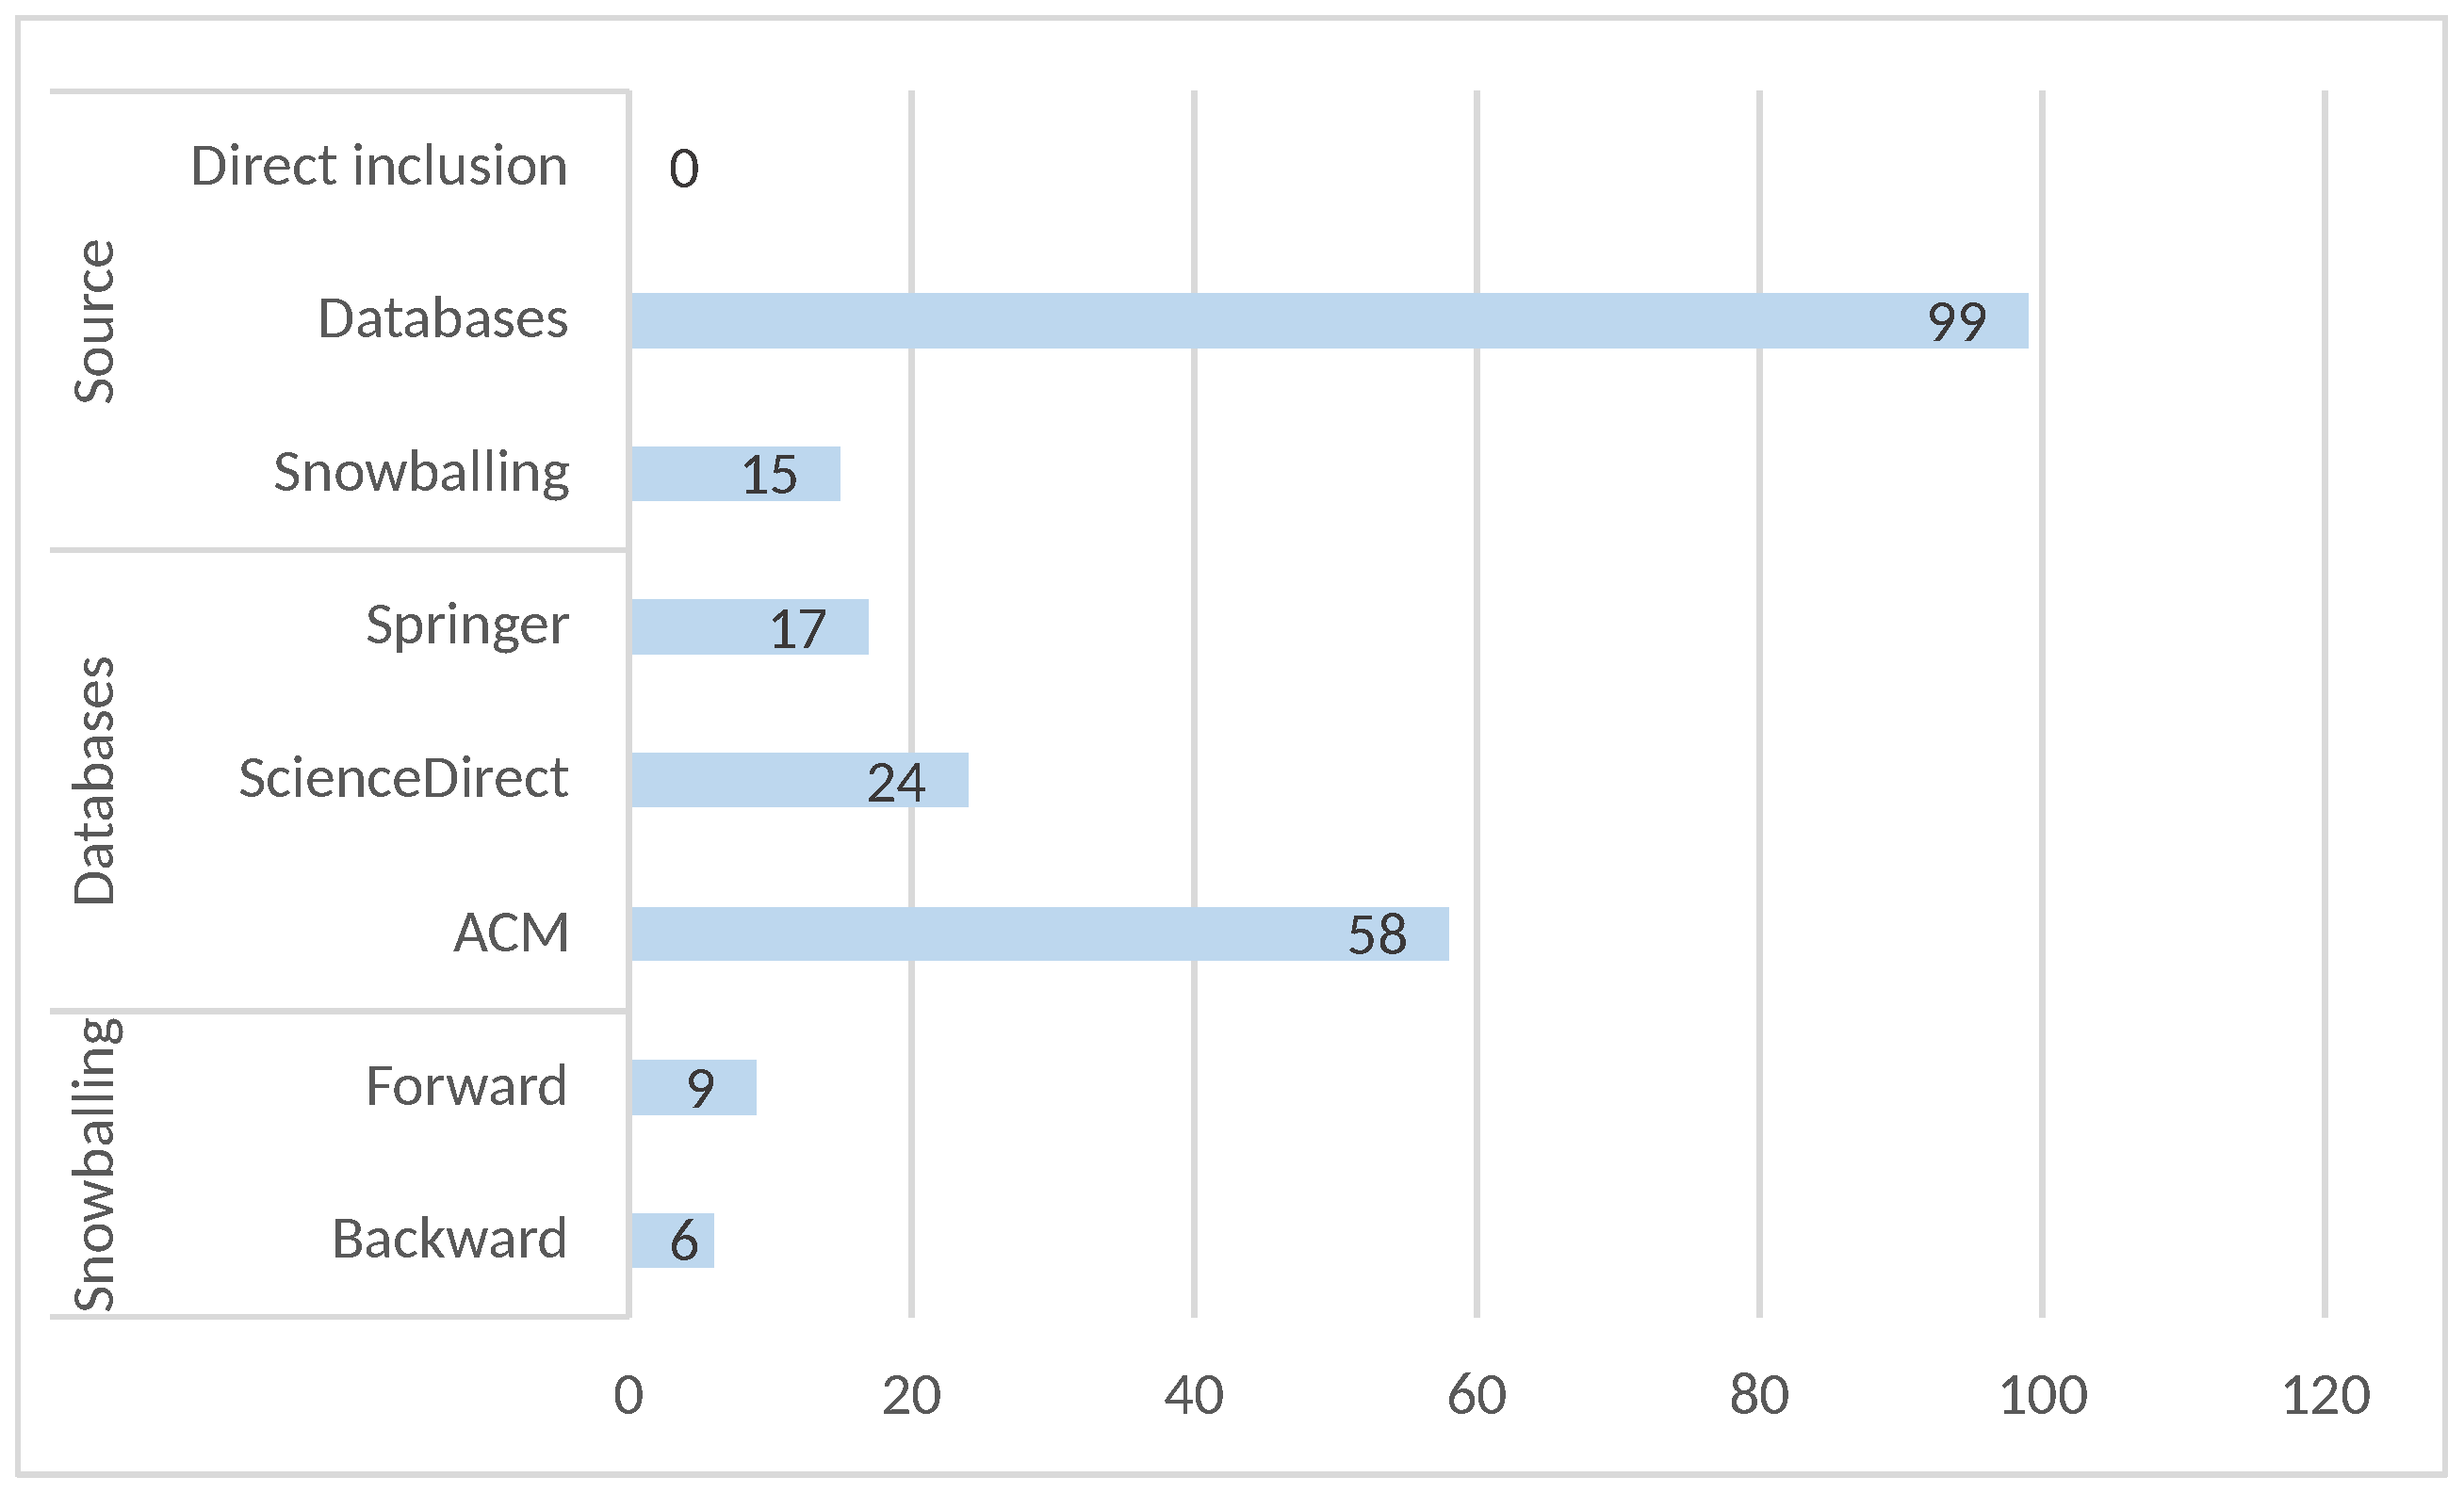
\includegraphics[scale=0.179]{resources/figures/Imagen1.eps}
	\caption{SPSs by source and search strategy.}
	\label{fig:SPSsByProcedence}
\end{figure}

These SPSs were obtained from digital databases, identified in the SMS through different strategies. Figure \ref{fig:SPSsByProcedence} shows the number of studies retrieved from various sources and the details of the database search and snowballing strategies. Regardless of the source, 86.84\% of the SPSs were found through database search, while the remaining 13.16\% were identified using the snowballing strategy.

Independent of the database search strategy, Figure \ref{fig:SPSsByProcedence} shows that of the 99 studies identified through database search, 58.58\% were found in the ACM database, 24.24\% in ScienceDirect, and 17.17\% in Springer. Among the 15 SPSs identified by snowballing, 40\% were discovered through backward snowballing and 60\% through forward snowballing.

\begin{figure}[ht]
	\centering
	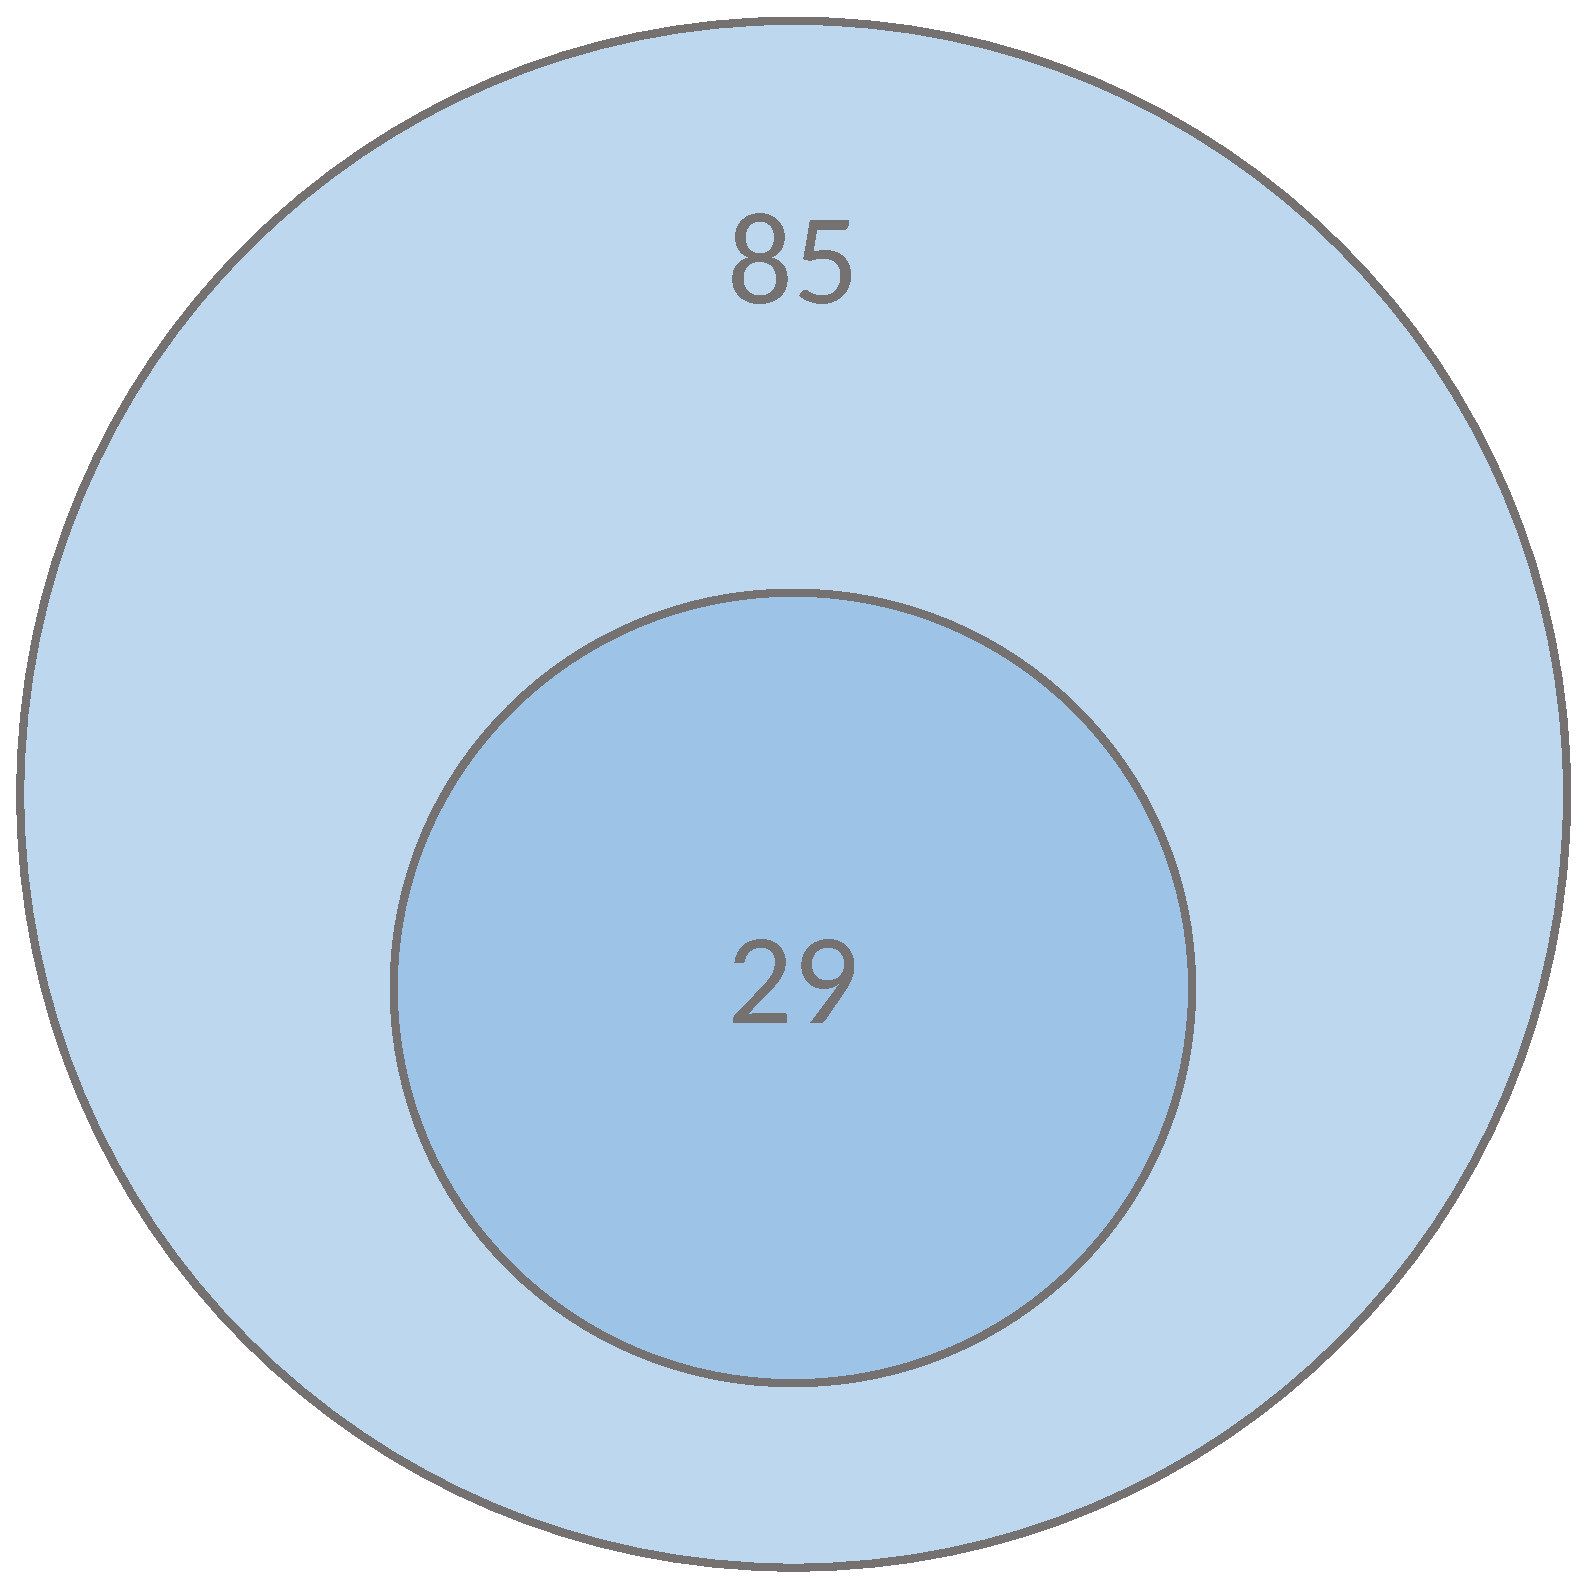
\includegraphics[scale=0.2]{resources/figures/Imagen2.eps}
	\caption{Relationship of SPSs with the research questions.}
	\label{fig:SPSsByRQs}
\end{figure}

Considering the relationships of the SPSs with the RQs, Figure \ref{fig:SPSsByRQs} shows that 100.00\% of the SPSs are related to RQ1, while 25.43\% of the SPSs are simultaneously related to both RQs. Consequently, the remaining 74.56\% are exclusively associated with RQ1. This indicates that no SPS is related solely to RQ2.

\begin{figure}[ht]
	\centering
	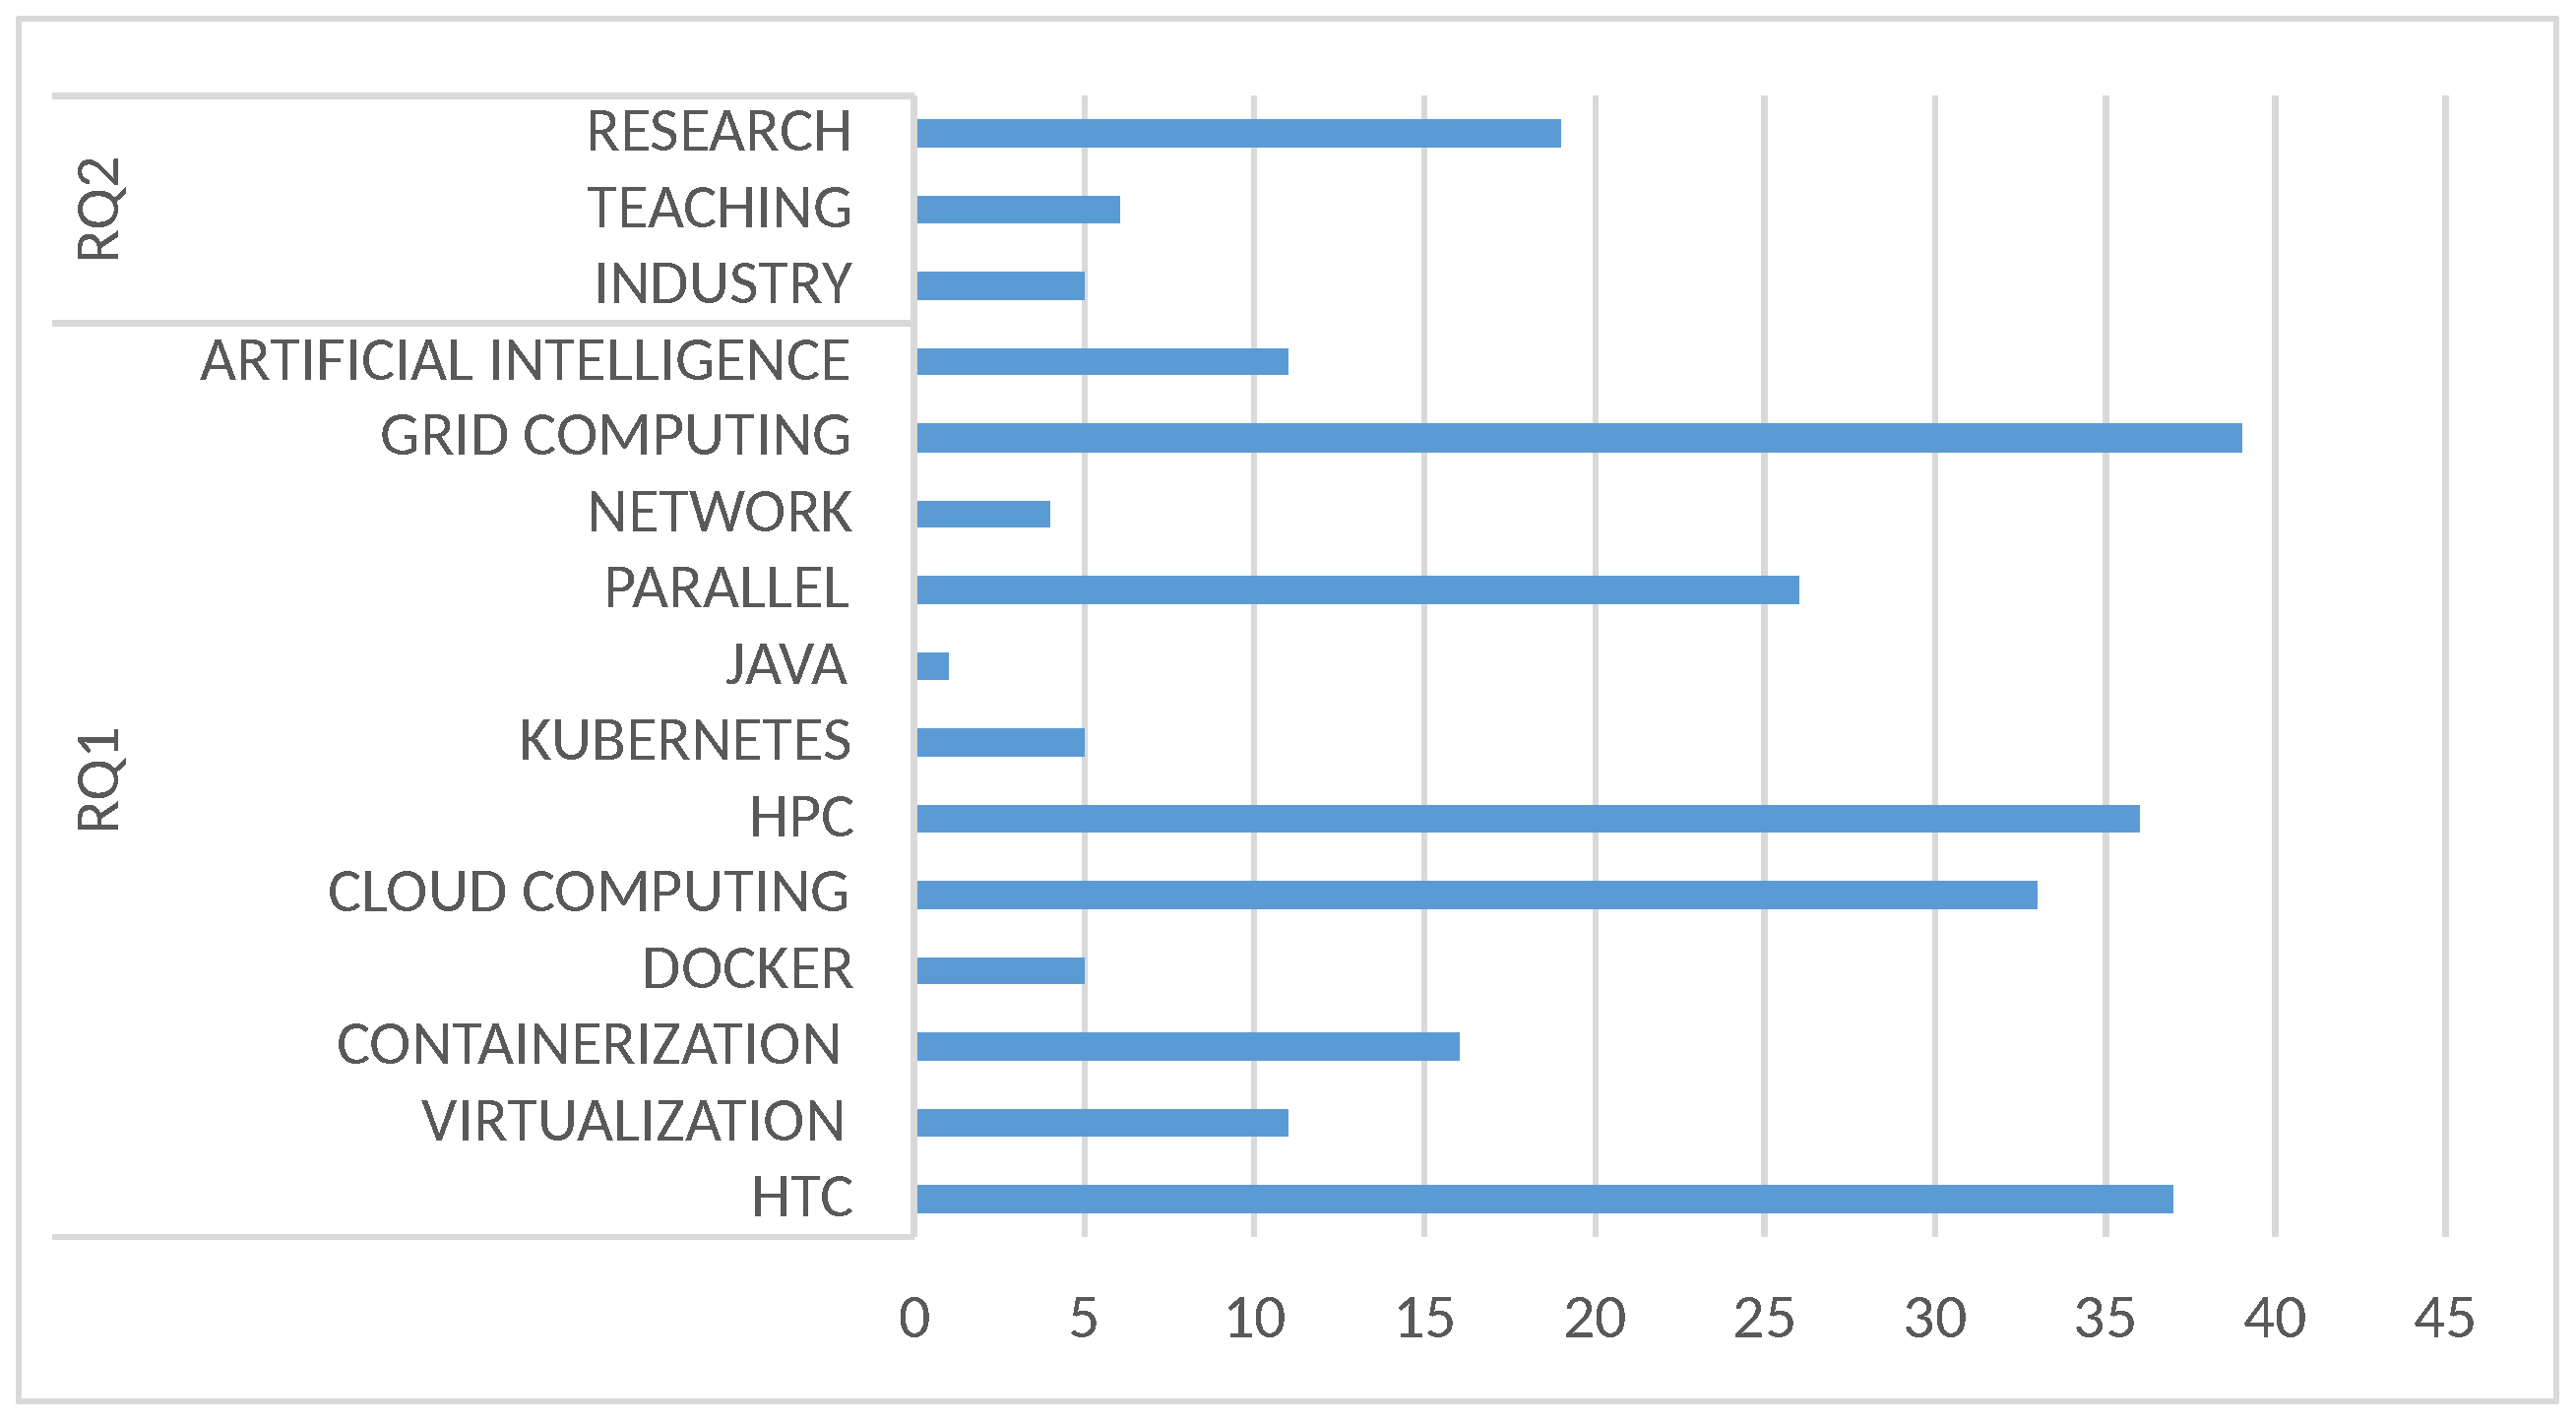
\includegraphics[scale=0.179]{resources/figures/Imagen3.eps}
	\caption{Relationship of SPSs with research topics.}
	\label{fig:SPSsByTopics}
\end{figure}

Figure \ref{fig:SPSsByTopics} shows the topics defined during the planning stage for each research question and the number of SPSs inclusively associated with each topic. It is essential to note that one SPS may be linked to multiple topics simultaneously. In this sense, Figure \ref{fig:SPSsByTopics} displays the 12 topics associated with RQ1, where the topic ``Grid Computing'' is the most frequent at 34.21\%. In contrast, the least frequent topic is ``Java'' at 0.88\%. On the other hand, Figure \ref{fig:SPSsByTopics} also shows the three topics associated with RQ2, where the topic ``Research'' is the most frequent at 16.67\%, while the least frequent is ``Industry'' at 4.38\%.

\begin{figure}[ht]
	\centering
	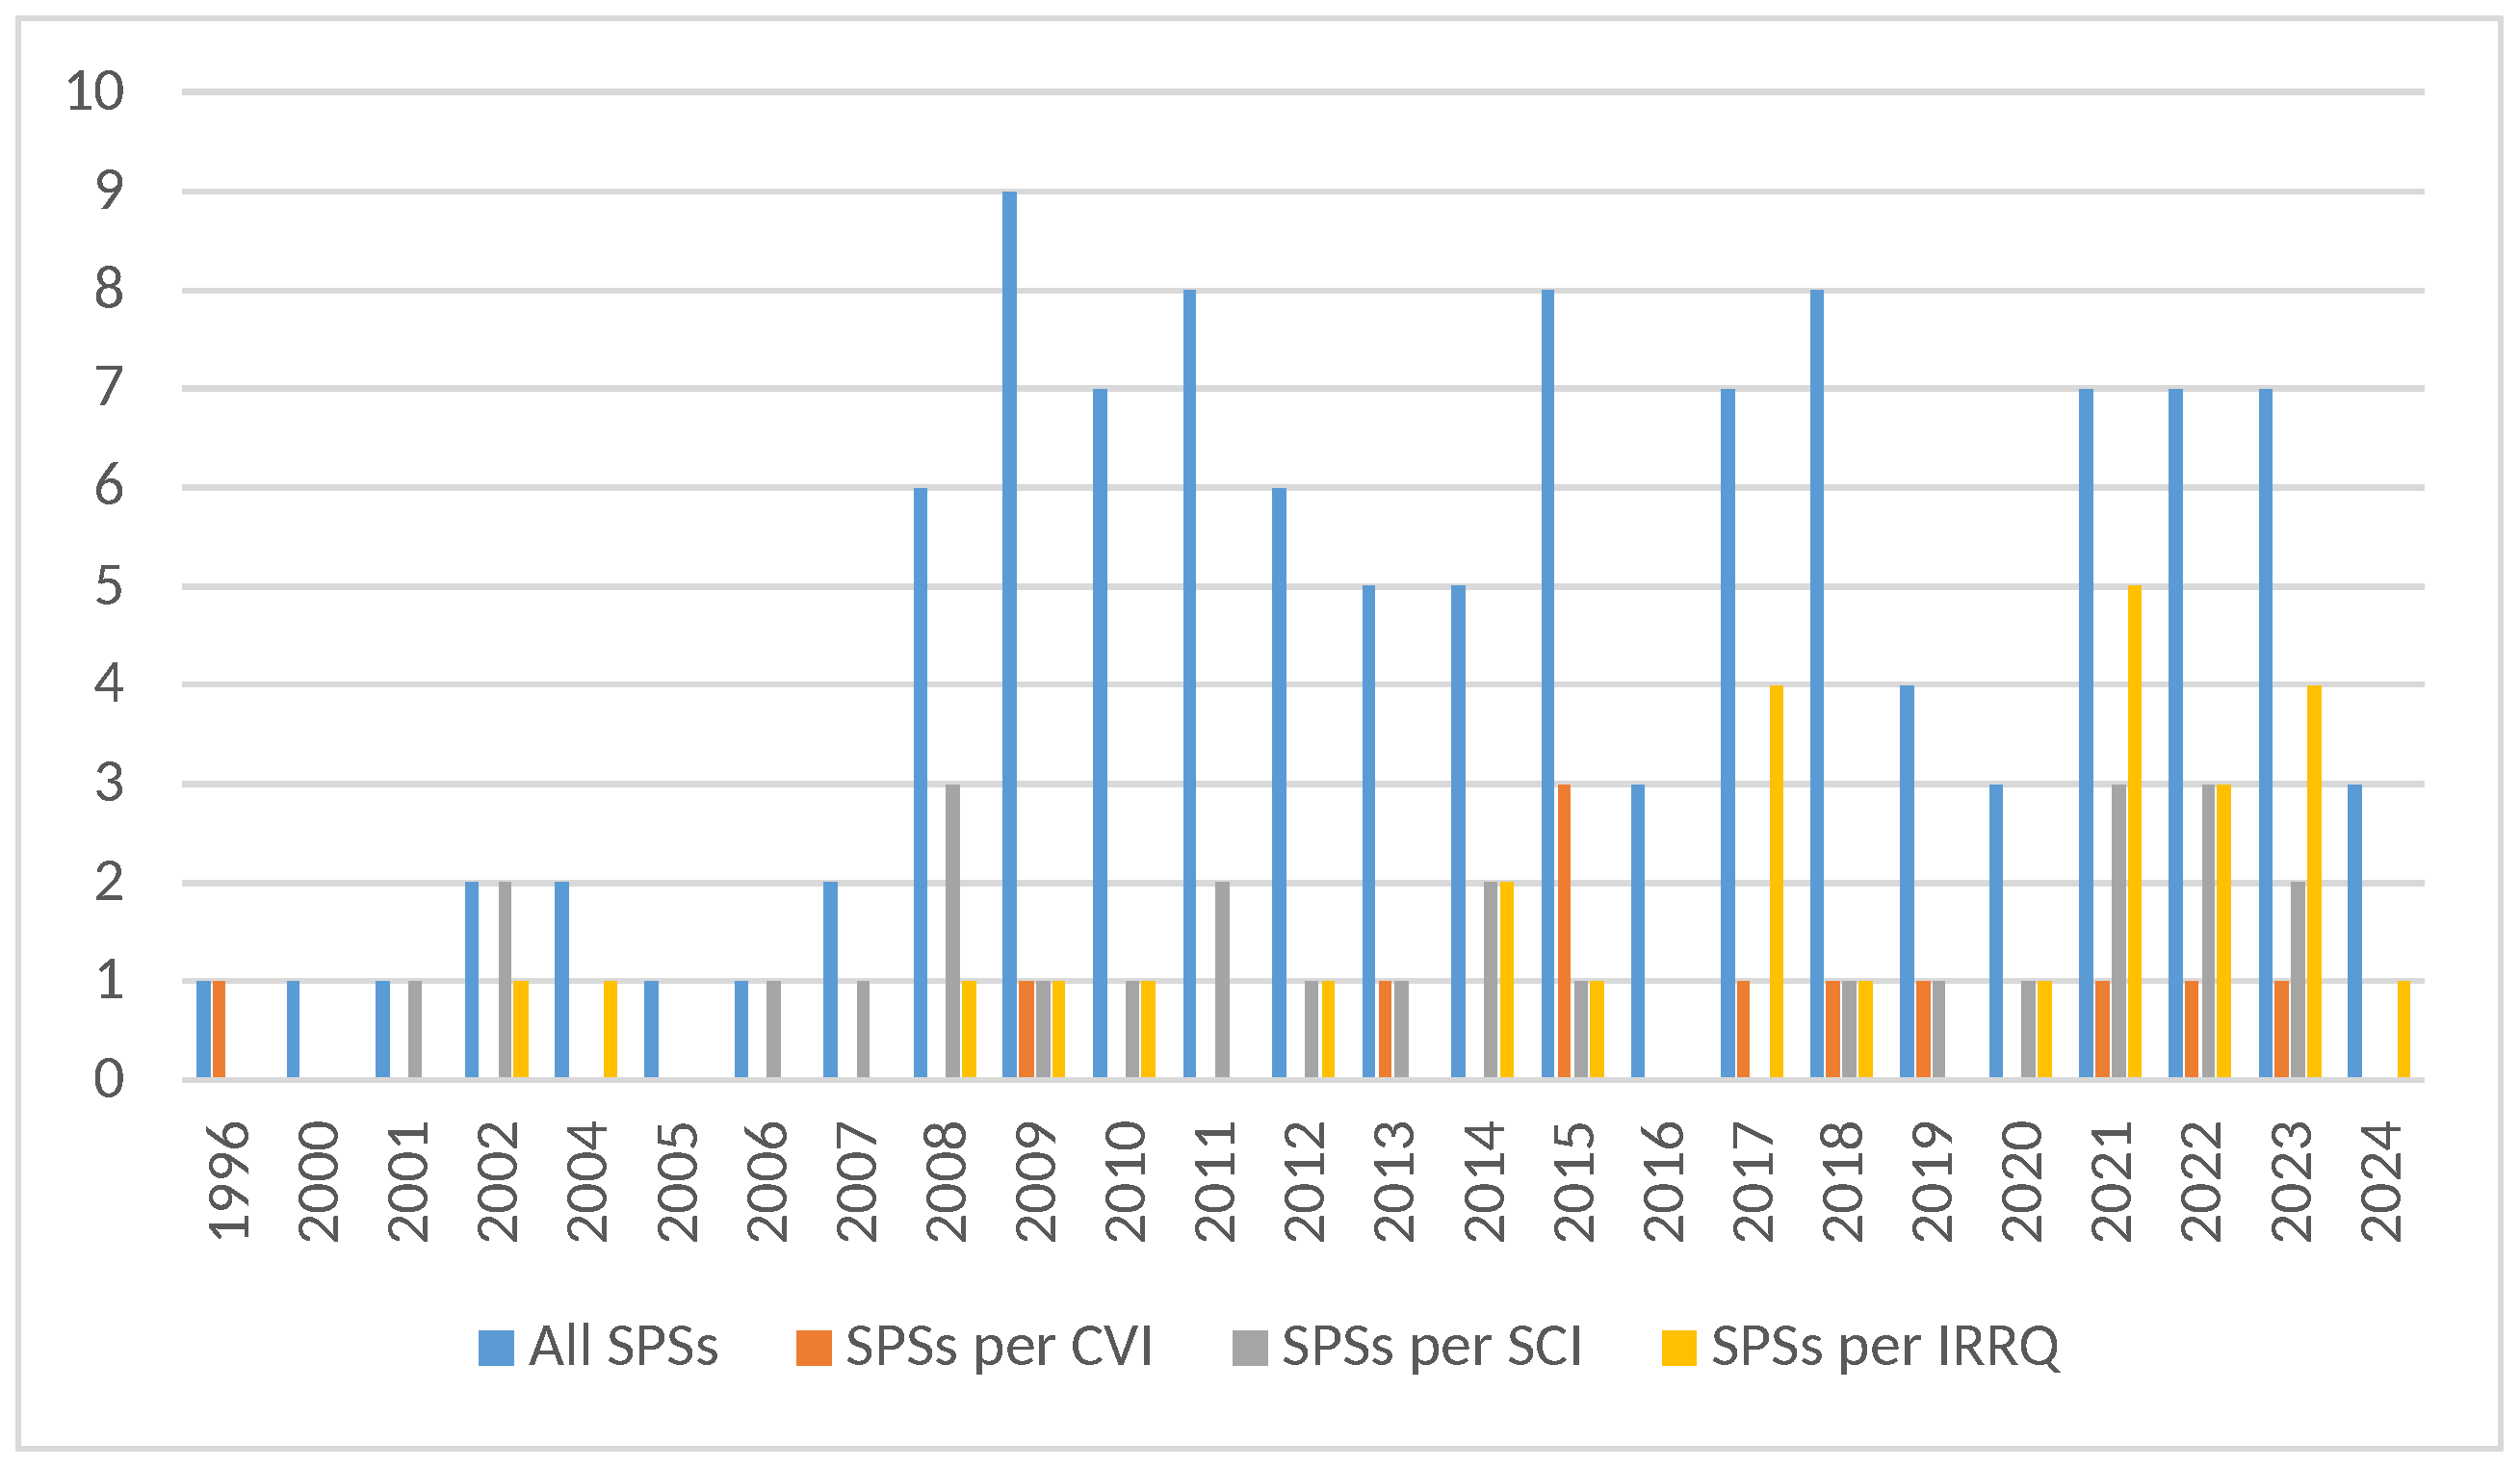
\includegraphics[scale=0.179]{resources/figures/Imagen4.eps}
	\caption{Relationship of SPSs with years of publication and quality indices.}
	\label{fig:SPSsByYearsAndIndexes}
\end{figure}

The studies publication period spans from 1996 to 2024. In this sense, Figure \ref{fig:SPSsByYearsAndIndexes} shows a low number of studies published between 1996 and 2007. In contrast, 2008 recorded an increase compared to 2007, with a total of 6 SPSs. The lowest number of SPSs was in 2009.

According to the SCI index, this SMS presents a relatively regular distribution across all years, with the exception of the period between 2006 and 2015, during which at least one SPS per year met the SCI index. Considering the distribution and the partially regular intervals in which no SPS met this index, this is regarded as an anomaly. Regarding the CVI index, the SMS shows regularity in the number of SPSs per year, particularly from 2017 onwards, except for the period between 2000 and 2008, when no SPS met the CVI index. Considering the IRRQ index, the year 2021 recorded the highest number of studies meeting this criterion, with a total of 5. Furthermore, there is evidence of a fairly consistent trend in the number of SPSs that satisfy this index over the years.

\begin{figure}[ht]
	\centering
	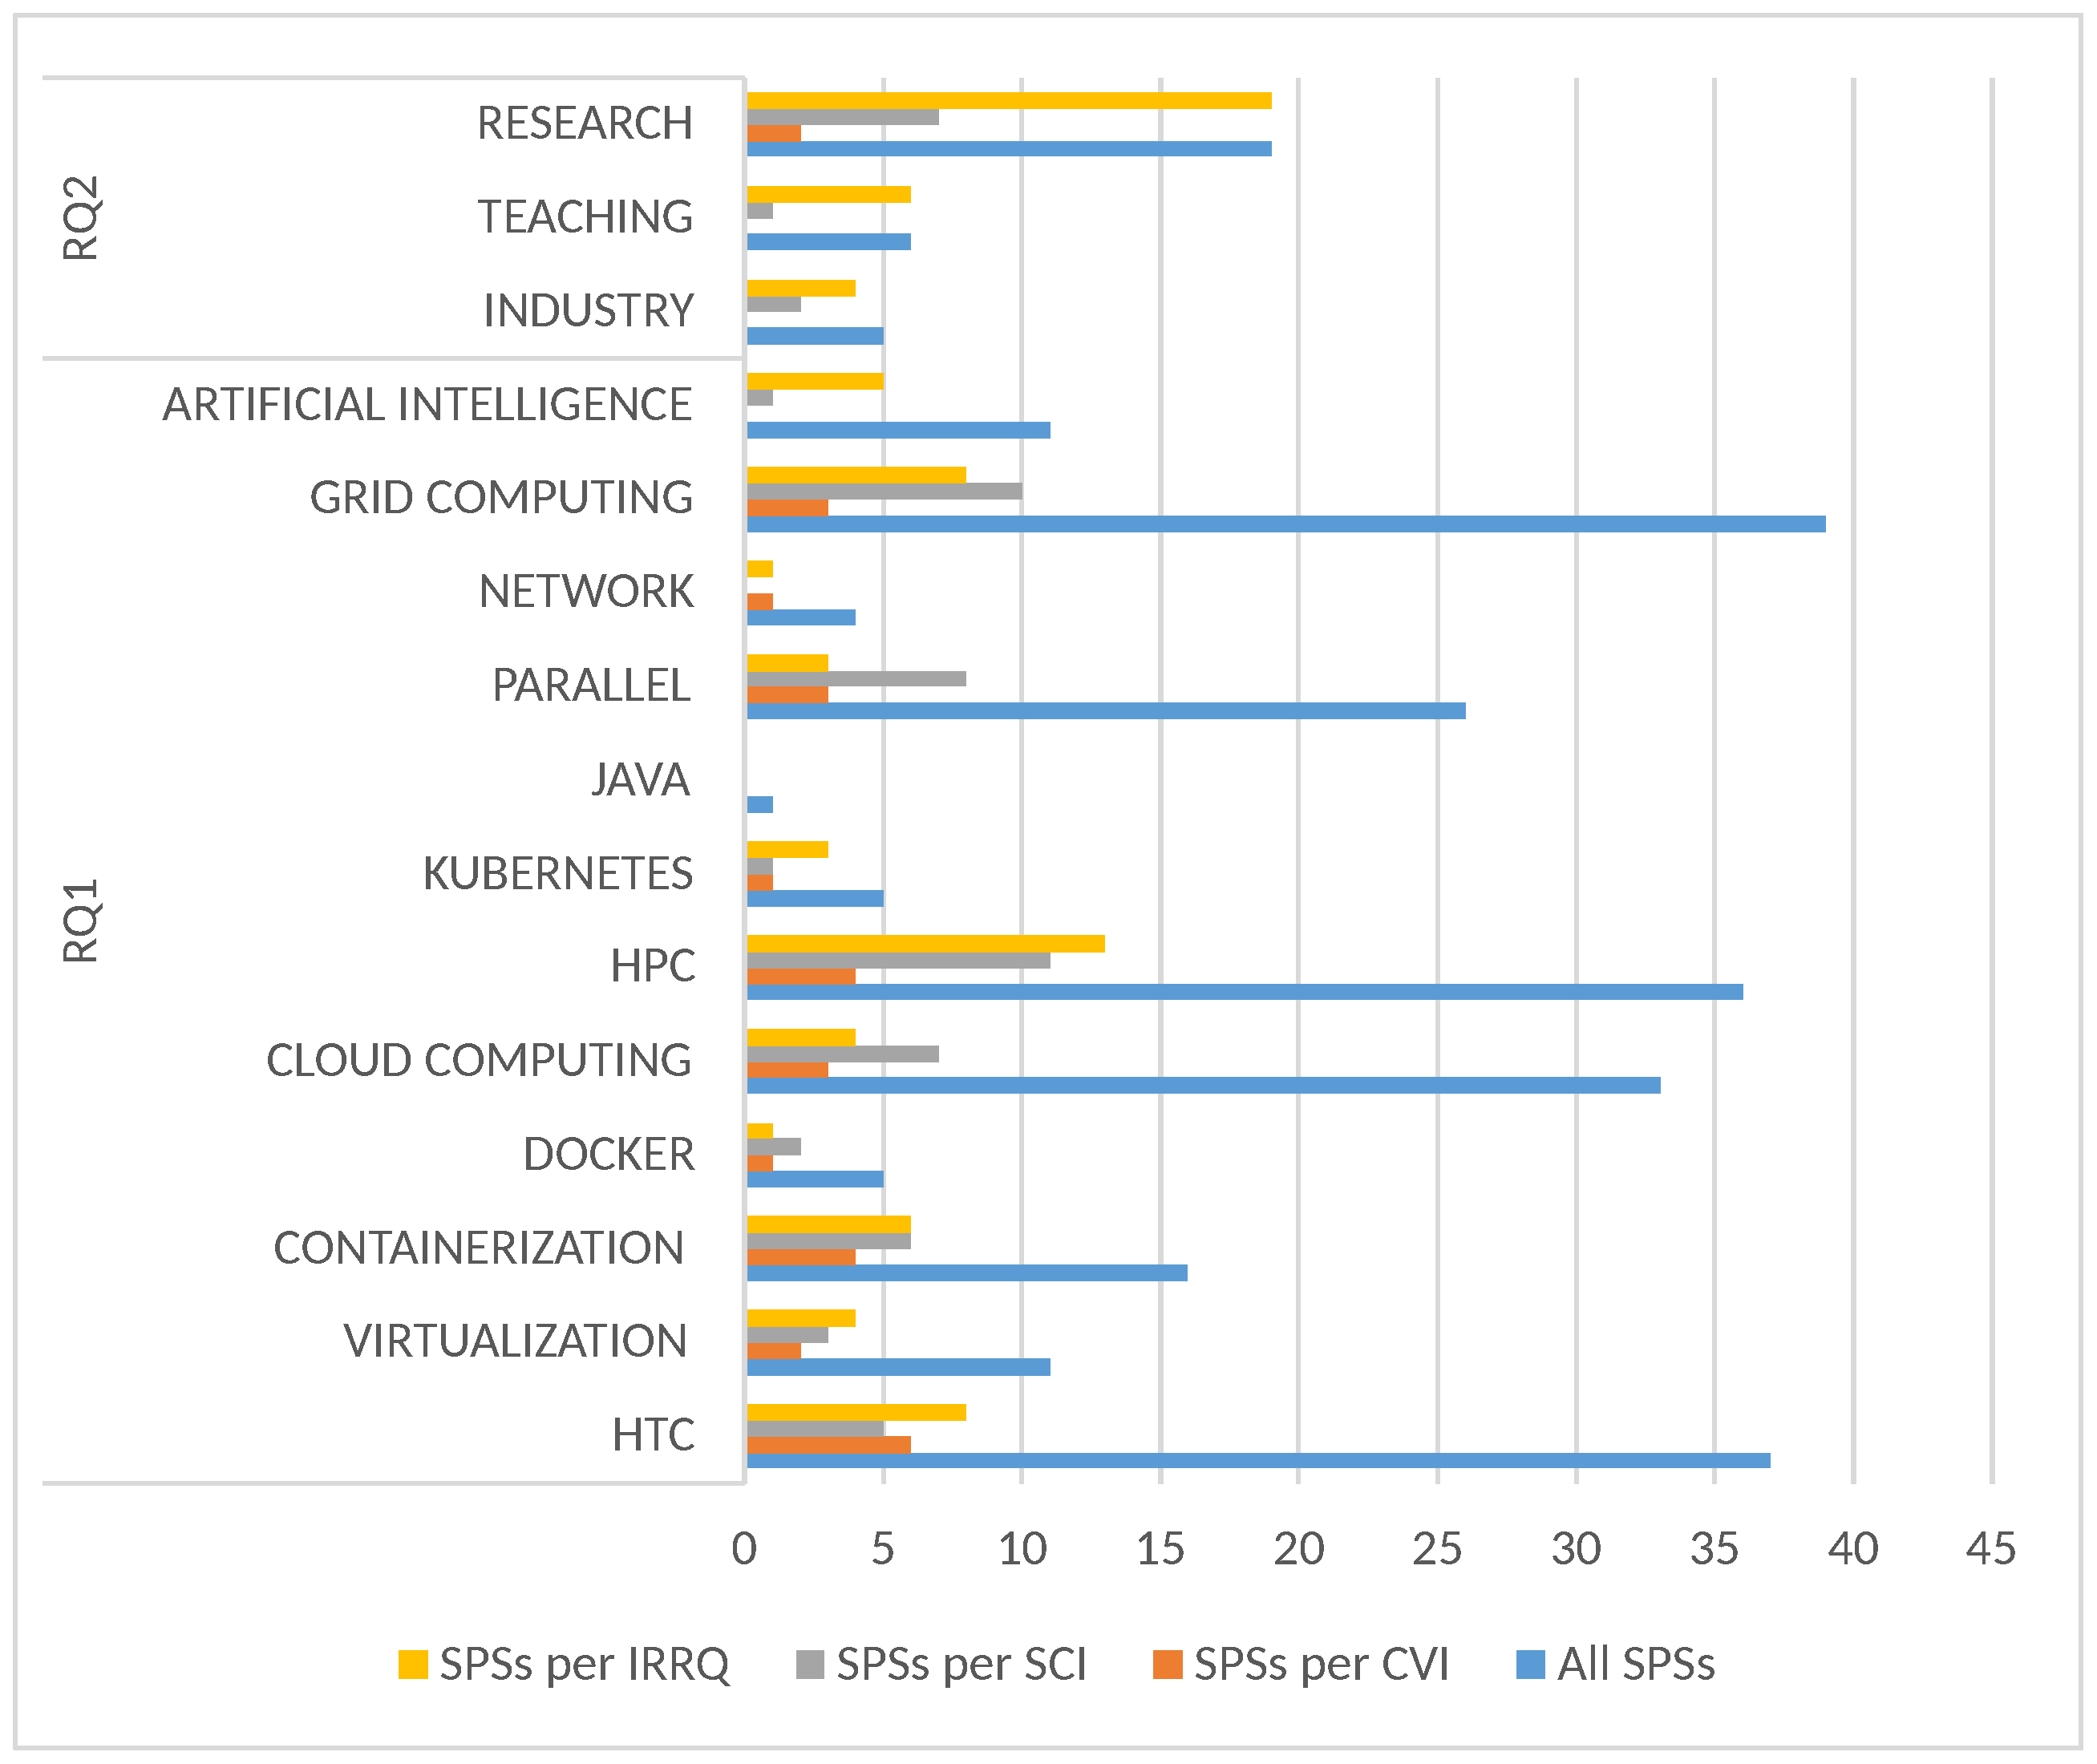
\includegraphics[scale=0.179]{resources/figures/Imagen5.eps}
	\caption{Quality indices by topic and research questions.}
	\label{fig:IndexesByTopicAndRQs}
\end{figure}

Figure \ref{fig:IndexesByTopicAndRQs} shows the number of SPSs classified by research question, including their respective topics and considering the quality indices.

In this sense, this study indicates that for RQ1, the topic ``Java'' registered the lowest number with 1 SPS, equivalent to 0.87\% of the 114 SPSs. In contrast, the topic ``Grid Computing'' is the most frequent with 39 SPSs, equivalent to 34.21\% of the 114 SPSs. On the other hand, for RQ2, the most frequent topic is ``Research'' with 19 SPSs, equivalent to 16.66\% of the 114 SPSs. Conversely, the least frequent topic is ``Industry'' with 5 SPSs, equivalent to 4.38\% of the 114 SPSs.

With respect to the CVI, SCI, and IRRQ indices, we identified the topics ``Java'', ``Network'' and ``Docker'' as the categories containing the fewest studies.

\begin{figure}[ht]
	\centering
	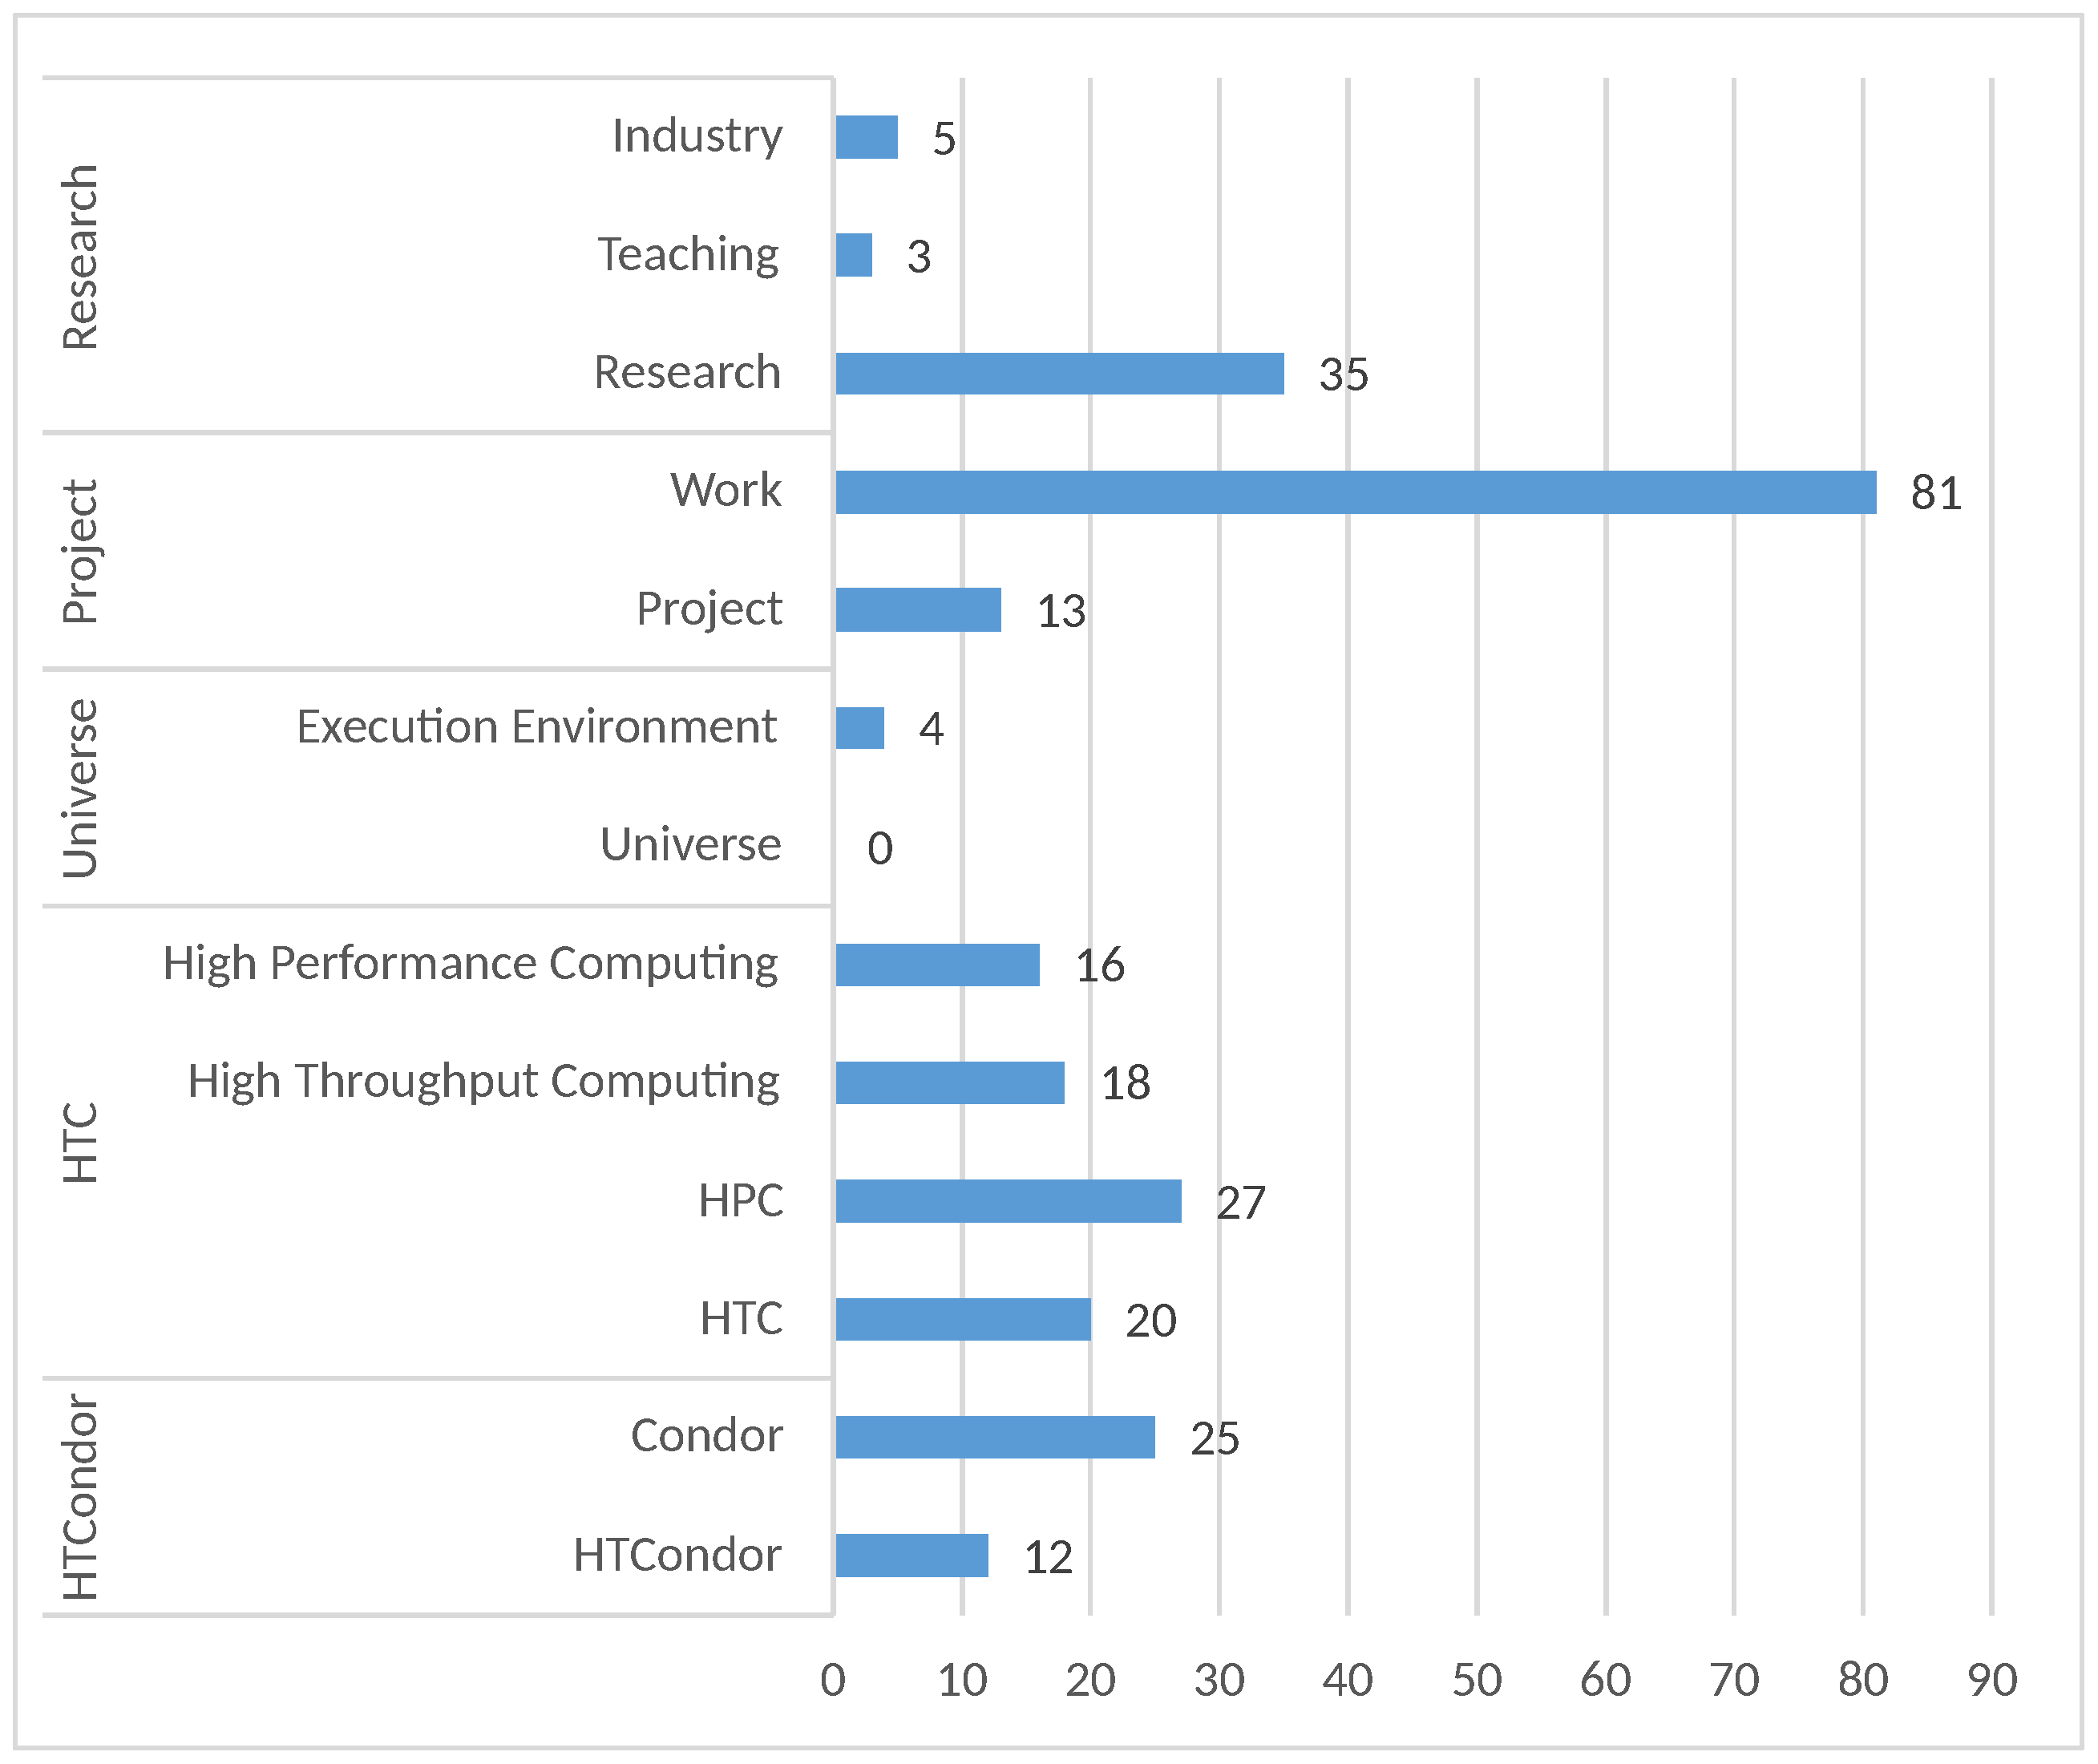
\includegraphics[scale=0.179]{resources/figures/Imagen6.eps}
	\caption{SPSs by keywords.}
	\label{fig:SPSsByKeywords}
\end{figure}

Figure \ref{fig:SPSsByKeywords} shows a cross-analysis between the SPSs, keywords, and synonyms. The synonym ``Work'' enabled the identification of 81 SPSs. Regarding the keyword ``Research'' it led to the identification of 35 SPSs. In contrast, the keyword ``Universe'' made the smallest contribution, resulting in the identification of no SPSs.

% sub-subsection 4.6.2
\subsubsection{Word Cloud Visualization}

\begin{figure}[ht]
	\centering
	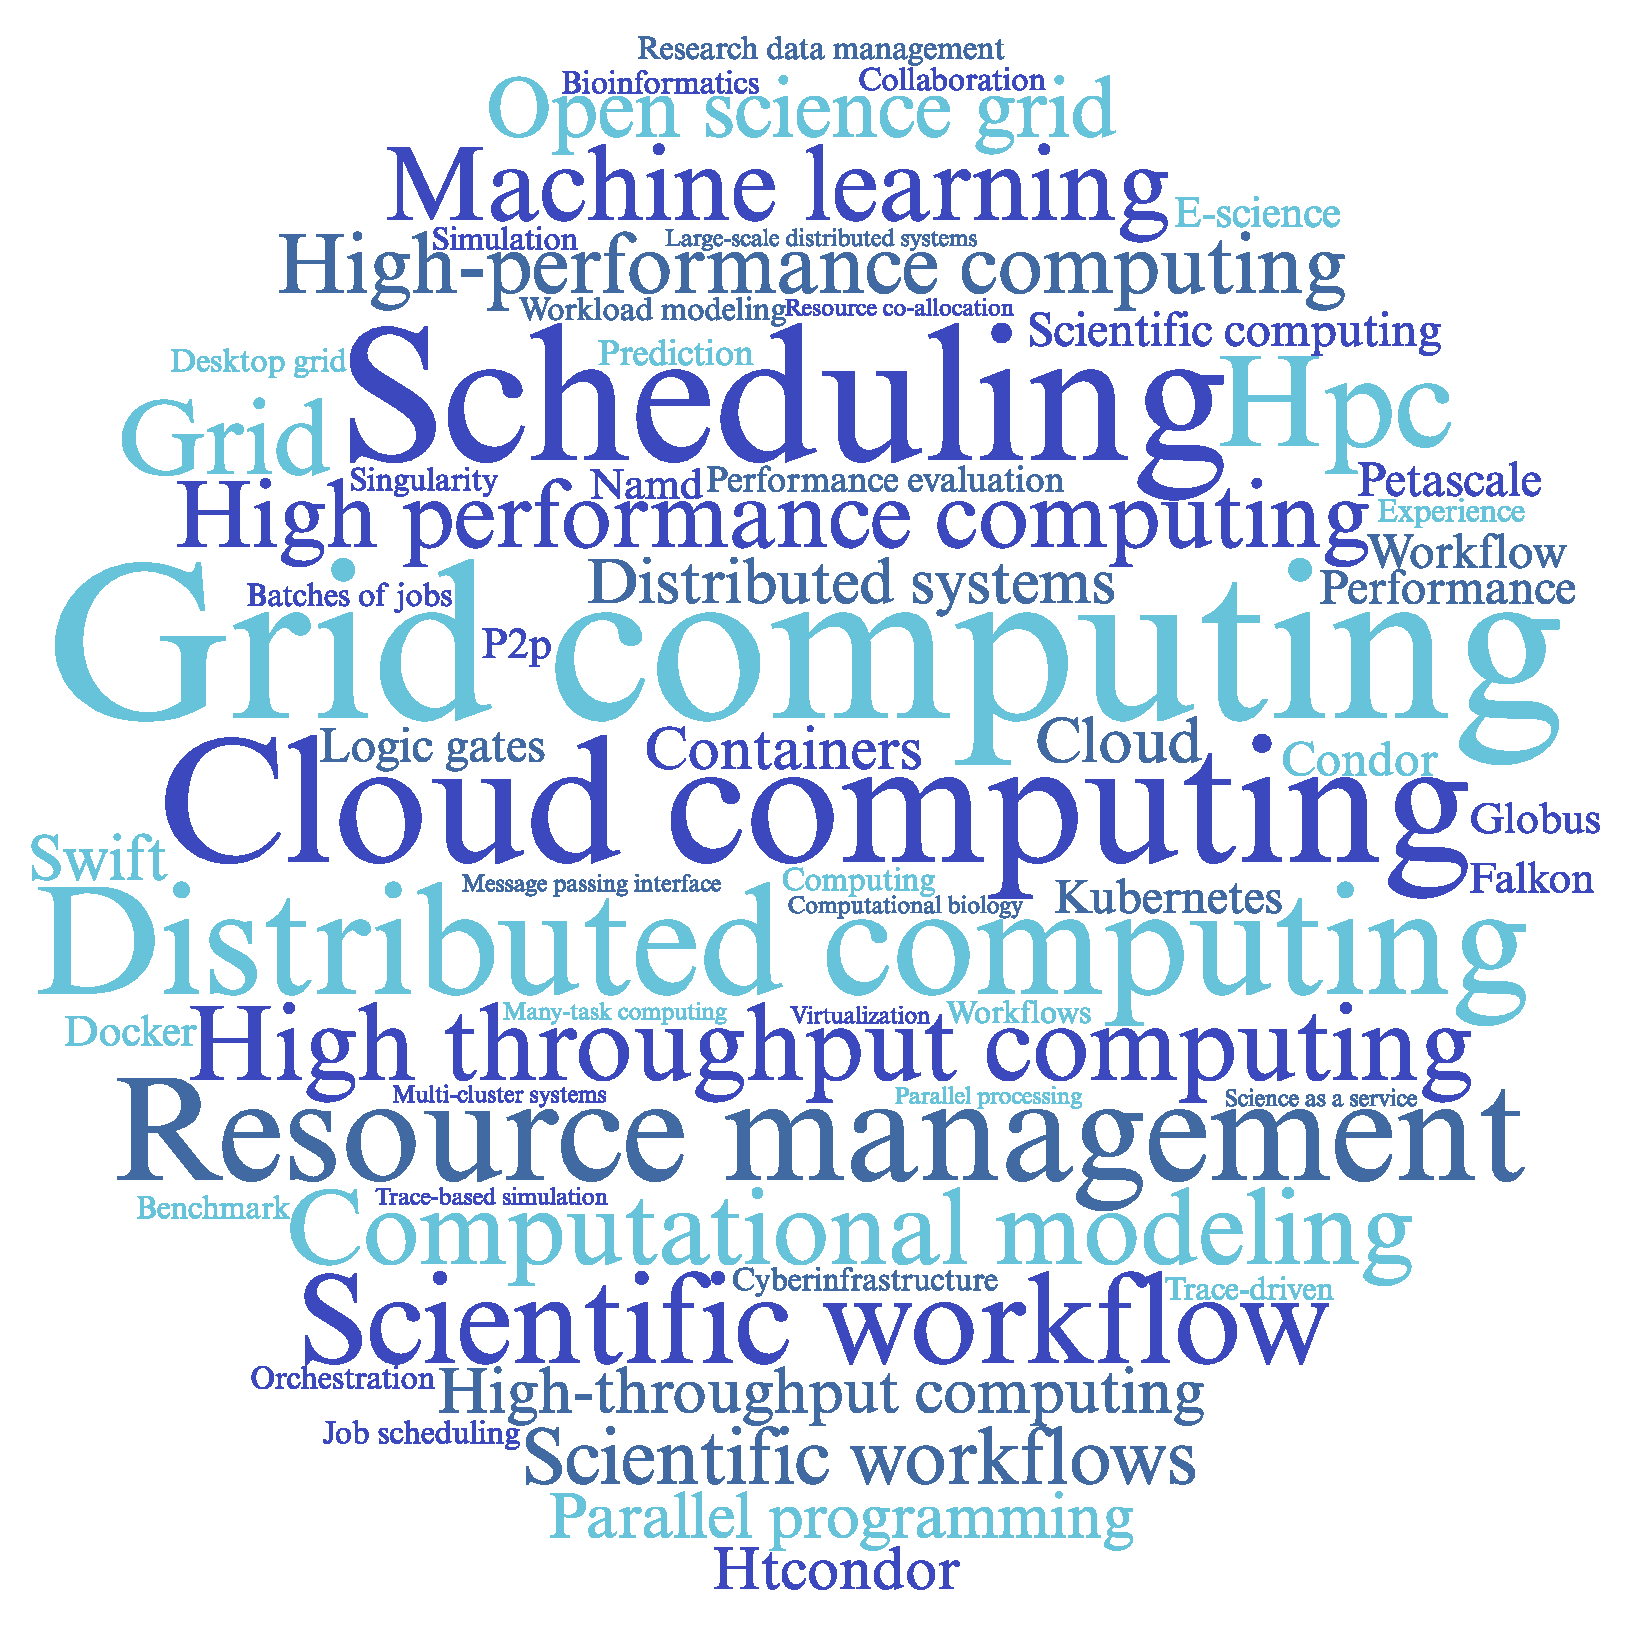
\includegraphics[scale=0.3]{resources/figures/wordcloud.eps}
	\caption{Word cloud of the keywords.}
	\label{fig:WordCloud}
\end{figure}

Another result obtained from the 114 SPSs of the SMS is the construction of a word cloud. This type of visualization seeks to highlight the most frequent and important words and concepts. Figure \ref{fig:WordCloud} shows the word cloud generated with the tool NubeDePalabras.es, built from the keywords of the SPSs.

Among the most frequent keywords, ``Cloud computing'', ``Grid computing'' and ``Distributed computing'' stand out, jointly contributing 18.59\% to the word cloud. The second level of relevance in terms of word cloud corresponds to ``HPC'', ``High Throughput Computing'' and ``Scheduling'' contributing 11.98\%. Finally, a third level includes ``Resource Management'', ``High Performance Computing'' and ``Scientific workflow'' contributing 7.85\%.

It should be emphasized that the calculations were made based on the words included in the cloud. In this case, all words with only one occurrence were excluded, so only words appearing at least twice were considered. This was done to extract the most relevant information. The percentages were then calculated based on the number of occurrences of the words with two or more appearances.
